\documentclass{article}
\usepackage[utf8]{inputenc}

%additional usepackages
\usepackage{amsmath}
\usepackage{eufrak}
\usepackage{tikz}
\usepackage{ amssymb }
\usepackage{import}
\usepackage[ruled,vlined]{algorithm2e}
\usepackage{booktabs}
\usepackage[capposition=top]{floatrow}
\usepackage{scrextend}
\usepackage{csquotes}
\usepackage{graphicx}
\usepackage{pdfpages}

\usepackage{caption}
\usepackage{subcaption}

% header
\usepackage{fancyhdr}

% bibliography
\usepackage[backend=biber, citestyle=authoryear]{biblatex}
\addbibresource{speciale.bib}

% functions

%\newcommand{\quickwordcount}[1]{%
%  \immediate\write18{texcount -1 -sum -merge -q #1.tex output.bbl > #1-words.sum }%
%  \input{#1-words.sum}%
%}

%\newcommand{\quickcharcount}[1]{%
%  \immediate\write18{texcount -1 -sum -merge -char -q #1.tex output.bbl > #1-chars.sum }%
%  \input{#1-chars.sum}(not including spaces)%
%}


%%%% INDEPDENT SIGN %%%%

\makeatletter
% Taken from http://ctan.org/pkg/centernot
\newcommand*{\centernot}{%
  \mathpalette\@centernot
}
\def\@centernot#1#2{%
  \mathrel{%
    \rlap{%
      \settowidth\dimen@{$\m@th#1{#2}$}%
      \kern.5\dimen@
      \settowidth\dimen@{$\m@th#1=$}%
      \kern-.5\dimen@
      $\m@th#1\not$%
    }%
    {#2}%
  }%
}
\makeatother

\newcommand{\independent}{\perp\mkern-9.5mu\perp}
\newcommand{\notindependent}{\centernot{\independent}}

\newcommand{\E}{\mathbb{E}}
\newcommand{\N}{\mathbb{N}}
\newcommand{\ndist}{\mathcal{N}}
\newcommand{\std}{\mathbf{std}}
\newcommand{\R}{\mathbb{R}}
\newcommand{\lra}{\Leftrightarrow}

\newcommand{\Loss}{\mathcal{L}}
\newcommand{\loss}{\mathcal{l}}

\newcommand{\la}{\leftarrow}
\newcommand{\ra}{\rightarrow}

\newcommand{\ones}{\mathbf{1}}

\newcommand{\statespace}{\mathcal{S}}
\newcommand{\actionspace}{\mathcal{A}}

\DeclareMathOperator*{\argmax}{arg\,max}
\DeclareMathOperator*{\argmin}{arg\,min}

% paranthesis

\newcommand{\lp}{\left(}
\newcommand{\rp}{\right)}
\newcommand{\lsp}{\left[}
\newcommand{\rsp}{\right]}
\newcommand{\lcp}{\left\{}
\newcommand{\rcp}{\right\}}

% Margins and paragraph indent etc (layout)

\setlength{\parindent}{0em}
\setlength{\parskip}{0.25cm}
\renewcommand{\baselinestretch}{1.5}
\usepackage[margin=1.05in]{geometry}

% header and footer

\pagestyle{fancy}
\fancyhf{}

\rhead{Jeppe Søndergaard Johansen}
\lfoot{\leftmark}
\rfoot{Page \thepage}


% About Data
\title{Deep Reinforcement Learning \& Dynamic Models}
\author{Jeppe Søndergaard Johansen (pcv439)}
\date{May 2020}

\makeindex




\begin{document}



\includepdf[pages={1}]{frontpage/frontpage.pdf}


\maketitle

%Number of characters: \quickcharcount{main}. Maximum is (144.000)

%Number of spaces: \quickwordcount{main}

\begin{abstract}
This paper investigates reinforcement learning as a solution method for dynamic models. A discrete time, finite horizon, discrete choice model of female labour supply and fertility is formulated, and the model is solved using value function iteration and two reinforcement learning methods, namely deep Q-learning and double deep Q-learning. After estimating the model using method of simulated moments, and finding the simple model inadequate to describe data from Statistic Denmark, the model is extended. The extension consists of 14 + 1 states. The extended model is solved only using double deep Q-learning and estimated using simulated method of moments. The results of the extended model convincingly matches data from Statistics Denmark and contemporary findings by \textcite{kleven_children_2019}. I conclude that the field of economics should further investigate reinforcement learning, as it allows solving dynamic models with high dimensional state space.
\end{abstract}


\pagebreak

\tableofcontents

\pagebreak

\section{Introduction} 

The last 10 years have lead to numerous breakthroughs within the field of machine learning, among them especially the subfield of reinforcement learning has experienced great leaps. In 2013 the company DeepMind achieved super human performance in various Atari games \parencite{mnih_playing_2013}. In 2018 the same company beat professional human players in the board game Go, a feat which was not deemed possible in a foreseeable future \parencite{silver_general_2018}, and as late as 2019 DeepMind showed that an reinforcement learning agent was able to play the game of Star Craft 2 on the same level as the best human players \parencite{vinyals_grandmaster_2019}. All the games mentioned can be considered dynamical models. Dynamic models play a central role within the field of economics. The results imply a new way of solving dynamic economic models using reinforcement learning.

Dynamical models usually involve agents that take sequential actions, trying to maximize the cumulative utility from these actions. This class of economic models conform to a set of properties economists like: They have a micro foundation - agents are utility maximizing. They model time, allowing for agents to foresee the future, and act in accordance to their expectations. Some dynamic models can be solved  analytically. This is true for the canonical Ramsey model. However when the scope of the dynamic model grows, different approaches is necessary. Dynamic programming is usually the tool utilized for solving such models.  Even though dynamic programming is a flexible tool it do have its limitations. Solving a model using dynamic programming, requires a limited sized state space, otherwise the computation involved becomes infeasible. In practice this leaves high dimensional dynamic models impossible to solve using contemporary techniques. Deep reinforcement learning allows for solving such models. Because these techniques are relatively novel, they have not yet been introduced into the field of economics. Deep reinforcement learning, does unfortunately not guarantee that the solution converges to the global maximum, but results have shown that learning is possible in hard, high dimensional environments.

This paper uses the aforementioned techniques to investigate the effect of children on female labour supply. Inspired by the model specification of \textcite{francesconi_joint_2002} and \textcite{adda_career_2011} I formulate an discrete time, finite horizon model that models discreet female labour supply and its relationship to fertility. First a simple model is formulated, where women can choose the number of supplied hours, letting fertility be exogenous, with an income process following the Mincer equation of human capital. The husband of the household, is assumed to follow a deterministic path both with regards to number of hours supplied to the labour force, and with the wage rates they receive. Households are assumed to face a budget constraint, that neither allow for borrowing or saving. Utility is assumed to be a function of leisure and consumption, and children are assumed to reduce leisure by mirroring additional work for the woman, that is not financially compensated. Later an extension to the original model is presented with exogenous education combined with a transfer system for women in the education system. Additionally the extension tracks children on an individual level.

Using three different solution methods: value function iteration, deep Q-learning and double deep Q-learning I solve the simple model. I show that one can get comparable performance using deep reinforcement learning compared to using value function iteration solution methods, yielding a new way to solve more complex dynamic models. The parameters of the Mincer equation are calibrated using data from Statistics Denmark . The model is estimated using method of simulated moments, where a simple grid search approach is applied due to fact the optimization problem being one dimensional. The extended model is only solved using double deep Q-learning. Again the model is estimated using method of simulated moments and grid search. The data used for the optimization is from Statistics Denmark.

My two main findings are: 1) Deep reinforcement learning can yield comparable performance to value function iteration solution methods. Considering this allows for solving dynamic models with high dimensional state space, I argue these methods should be explored further in the field of economics. 2) Simulating from the estimated model, I find the initial simple model is not able fit the data, whereas the extended model does fit the data surprisingly well. Both participation rates and average number of supplied hours to labour force, are surprisingly close to what the data from Statistics Denmark suggest. Comparing to  \textcite{kleven_children_2019}, this paper finds results very similar with regards to earnings, participation rate, supplied hours to the labour force and wage rates, when women gives birth to a child.

The paper follows the structure: A literature review is conducted highlighting the main findings and articles of endogenous female labour supply and the effect of children. A model is formulated based on key takeaways from the literature. The parameters of the income process is calibrated using data from Statistics Denmark. Next, I introduce the reader to both reinforcement learning and deep learning. Settling on three different solution methods i solve and estimate the model. I go on to extend the model, and solve it using double deep Q-Learning. I end by comparing the results to contemporary findings, and data from Statistics Denmark.

\section{Review of Literature}\label{sec:lit_review}

There exists a deep literature on both labour supply and fertility.
As this paper tries to investigate the relationship between women's labour supply and fertility by formulating a dynamic  structural model, the focus will lie on literature that has the same scope. The paper that has been the main inspiration for this paper has been work by \textcite{francesconi_joint_2002}, where he proposes a joint dynamic model of fertility and labour supply of married women. Francesconi formulates a model with a joint decision of fertility and labour supply. Labour supply is considered in his formulation split into three choices: not work, work part-time and work full-time. Furthermore Francesconi proposes a model of human capital accumulation as a function of the labour supply. Additionally he assumes a budget constraint of all income in period $t$ should be consumed in period $t$, and the husbands income and labour supply is modelled to follow an exogenous process.  main findings of the paper is that a clear relationship between earnings ability and preference for work, where women with highest earnings profiles negatively, has the lowest marginal utility of children.

Work has also been done in extending the basic framework proposed by \textcite{francesconi_joint_2002} that models joint decision between fertility and labour supply.  \textcite{adda_career_2011} extends the life cycle model by allowing for savings, and more sophisticated skill atrophy processes,  \textcite{gayle_life-cyle_2006} allows for the participation rate of women to be continuous and \textcite{keane_role_2010} focuses on the marriage market while still allowing for fertility and labour supply being part of the choice set. \textcite{adda_career_2011} suggest that fertility might be falling in developed countries due to significant cost to the careers and future earnings of women. They find that the cost of career interruptions as a consequence of children, is non-linear over the career cycle and has the biggest impact around mid-career. They also find that children has influence on career planning, and the effect of planning to have children, affects the career even before the first child. \textcite{gayle_life-cyle_2006} employ a semi-parametric approach to a panel data setting. Inline with \textcite{francesconi_joint_2002}, \textcite{gayle_life-cyle_2006} finds that having children is less desirable for women on high income trajectories. \textcite{keane_role_2010} finds that differences in skill rental price between black and white women can explain the number of teenage pregnancies, implying again that a relationship between fertility and career trajectories is present.

The joint decision between fertility and labour supply has been investigated before \textcite{francesconi_joint_2002} investigated the problem by proposing a dynamic structural model. Both \textcite{moffitt_estimation_1984} and \textcite{hotz_empirical_1988} utilizes an closed form approach to the problem of fertility and labour supply to estimate an econometric model. \textcite{moffitt_estimation_1984} employs a cross sectional approach and finds that he is able to better fit the bimodal distribution of working hours. While controlling for number of children he finds that more children in general imply women work less. \textcite{hotz_empirical_1988} makes the interessting addition to their model, that fertility is only somewhat a choice of the household, i.e. with some probability the fertility outcome will diverge from the household's expectation. They find that maternal time required for a newborn child is 660 hours per year, decreasing geometrically as the child ages. They also find that children do not reduce a woman's labour supply 1-to-1, rather the time spend on children will be taken from other activities as well.

Looking to the effect of children on labour supply has been investigated by \textcite{angrist_children_1996} finding that, the effect of children on labour supply disappear as the child turns 13. The paper emphasizes the causal link (using IV-estimation) between fertility and labour supply and finds that fertility only have a small effect on the labour supply of women. Considering the effect of children  \textcite{altug_effect_1998} employs a semi-parametric approach to estimating the effect of experience on female labour supple, controlling for children. They find that the impact of children on women's participation rate is ambiguous, but for married women, additional children increases number of hours worked.

\textcite{attanasio_explaining_2008} proposes a structural model, that investigates the extensive margin of women that work, leading them to a formulation where women can either work or not work. Their main addition to their model is letting the households borrow, separating them from \textcite{francesconi_joint_2002} among other earlier studies, that did not allow for such behavior. Human capital is accumulated when women enters the work force. They investigate 3 cohorts (Dole, Clinton and Oprah) as to see the what can account for their different participation rates. Their main finding is that some of the difference can be explained by reduced child-care costs and a reduction in the wage gender gap. A later paper from the same authors \textcite{attanasio_aggregating_2018} they construct a model where they again investigate the participation rate of women. In this formulation they control for family composition and importantly include to "taste-shifters" in the utility function. These are latent variables that us used to explain how the participation rate can change under different circumstances. Their main finding is that heterogeneity of demographics, wealth distribution and the point of the business cycle can explain a lot of the aggregate responses of female labour supply.

\textcite{del_boca_motherhood_2009} investigates uses cross-country European data to investigate the join decision about fertility and labour market participation. They control for personal characteristics as well as childcare system, parental leave system, family allowances as well as part time opportunities. Their main findings include that labour market and social environment do not affect fertility in a significant way. They find however that the institutions that can support women's labour market participation does indeed have impact on the women's labour market participation, especially this effect is the most present in less educated women. These results are somewhat in line with \textcite{haan_can_2009} that investigates the impact of financial incentives on female labour supply by exploiting the variance stemming from the tax and transfer system. They also find that child care subsidies do increase labour supply, however in contrast with \textcite{del_boca_motherhood_2009} they do find that child care subsidies do increase fertility as well.

\textcite{jones_fertility_2008} makes a comparative analysis of the prevalent theories explaining the relationship between fertility and income: whether it is taste or ability that can explain the differences in income. They find that both theories can explain, however the ability hypothesis can only hold under the assumption of a elasticity of substitution between consumption and the number of children. Therefore they conclude that the taste theory is more robust.

\textcite{blundell_female_2016} uses quasi-experiment of the UK tax and welfare reforms of the 1990s and 2000s to investigate women's labour supply. They construct a dynamic model where women can save and accumulate human capital, along with educaiton. They make the women choose education level and their participation rate in the labour market. In contrast with \textcite{francesconi_joint_2002} they do not let fertility be part of the choice space, rather they model it as a random event. They control for demographics etc. They find that labour supply elasticities are generally high (but below 1), except for single mother that seem to have above 1. Another interesting result from the paper is that tax credits do seem to let low-education women into the workforce, however it does not seem to have long term influence on employment or wages for this group. \textcite{eckstein_dynamic_2011} also investigates the discrepancy between lone mothers and married couples by constructing a dynamic life cycle model, their motivation being that while the labour supply of women the last 50 years have had a sharp rising trend, the same cannot be said for unmarried women\footnote{Married women has a gone from 30\% to 60\% employment, where single and divorced women have been at around 70\% employment throughout the sample.}. The authors conclude that the rise in female employment in large part can be explained by the increase in years of schooling and the rise of female wages. They also find that changes in fertility and marital status do not have a big impact. 

Briefly discussing results in a danish context, using Danish data \textcite{kleven_children_2019}. They do find that the long term effects of the arrival of a child reduces earnings by about 20 \%, and the hours worked by 10\% for women, while no effects are notable for men (10 year horizon). The same goes for participation rates which fall about 13 \% and wage rates which falls about 9 \% in the long run for women (10 year horizon). \textcite{jorgensen_life-cycle_2017} investigates the relationship between consumption of non-durable goods and the average number of children, since these follows the same trajectory over the life cycle. He finds that income of the households fall significantly, but in contrast with \textcite{kleven_children_2019} the economic effect is negligible at around 1\% reduction in households with one child compared to households with no children. 

\section{Model specification}\label{sec:model1}

This paper presents a discrete time, finite horizon, discrete choice model of female labour supply. More specifically I model a household consisting of wife, husband and a zero or more children. The model attempts to address what the effect of children is on the labour supply of women. The model consists of 3 components: 1) An income and human capital component, 2) A fertility process, 3) A leisure and utility component. I model the households from age $Q_{min}=18$ to the terminal age $Q_{max} = 60$. Here it should be noted, that I make the simplifying assumption that the husband and wife has the same age and that the couple is married from age $Q=18$. The age evolves in a deterministic fashion, i.e. the household grows one year older for each step in the model:

\begin{equation}
    Q_{t+1} = Q_t + 1
\end{equation}

For each time step in the model, the agent has to  choose how many hours the woman of the household should supply on a weekly basis. The choice is discreet, and consists of four action values: $H_t \in \{0, 25, 37, 45 \}$. The labour supply of the man in the households is not a choice variable and is therefore considered an exogenous variable.

The households has two income streams, the husband, which is perfectly deterministic, and the wife. The income process of the wife consists of an idiosyncratic component $Z_t$, which follows a random walk:

\begin{equation}
    Z_{t+1} = Z_t + \epsilon_t, \qquad \epsilon_t \sim \ndist (0, \sigma_\epsilon)
\end{equation}

This allows for agents to do display heterogeneity owing to the fact that some unobserved carrier choices will lead to higher wages, even though two otherwise identical agents have been part of the labour force equally long. Since these job characteristics is unobserved, it is assumed to be a random walk. The second component of the income process is a human capital component based on the Mincer equation, as described by \textcite{lemieux_mincer_2006}. That is the the log-transformed wage rate/wage level can be described by the human capital accumulated:

\begin{equation}
    \log \tilde{W}_t = \alpha + \eta_G G_t + \eta_{G^2} G_t^2
\end{equation}

A couple of things to note. In the original formulation by \textcite{lemieux_mincer_2006}, the education level is also included. However, due to the lack of availability of such data I am not able to condition on this. It should also be noted, that the state $G_t$ represents the human capital accumulated of the woman in the household. Finally this equation governs only the wage rage of the women (not of the husband), for whom the wage rate and the supplied number of hours is considered exogenous. The exogenous wage rate of the husband is found using the data set \textbf{LONS50} from Statistics Denmark. And the number of supplied hours for the husband is found using the data set \textbf{LIGEF15}, again supplied by Statistics Denmark. The wage rate of the women will be capped at the minimum wage if the sum of the two components $\tilde{W}_t + Z_t$ is not above the the minimum wage $W_{min} = 120$: 

\begin{equation}
    W_t = \max ( W_{min}, \tilde{W} + Z_t)
\end{equation}

The human capital accumulation process, follows a formulation allowing for depreciation (or skill atrophy):

\begin{equation}
    G_{t+1} = G_t (1-\delta)  + \frac{1}{37} H_t 
\end{equation}

Where 37 being the standard number of hours worked in Denmark. The total income $Y_t$ of the household can now be formulated as:

\begin{equation}
    Y_t = 46 \cdot W_t \cdot H_t + f^M(Q_t)
\end{equation}

Where $f^M$ represents the income from the husband as a function of age. And $46 \cdot W_t \cdot H_t$ is the number of supplied hours pr. week, $H_t$, times the number of weeks, 46, in a year for the average person on the labour market\footnote{Assuming 6 weeks of holiday.} times the wage rate, $W_t$. The income process is a function of the number of supplied working hours, $H_t$, and the states $(Q_t, Z_t, G_t)$. The parameters $\delta, \sigma_\epsilon, \eta_G, \eta_{G^{2}}$ will be calibrated in section \ref{sec:parameter_calibration}.

The second component of the model is the fertility process. The fertility is assumed to be exogenous depending on the age of the woman. This is summed up in the equation below:

\begin{equation}
    K_{t+1} = K_t+ \psi_t, \qquad \psi_t \mid Q_t \sim Bernoulli (p_\psi(Q_t))
\end{equation}

$K_t$ is the number of children in the household. The household is assumed to start with $K_t = 0$ at age $Q=18$. At each step with probability $p_\psi(Q_t)$ the wife gives birth to a child. Allowing for the accumulation of children. The number of children is capped at a maximum of 5 in the model. The probability $p_\psi(Q_t)$ is modelled using data from Statistics Denmark using the data set \textbf{FOD33}. The number of children $K_t$ is part of the state space. 

The third component of the model is the utility and leisure component. The agent is assumed to get utility from leisure, $L_t$, and consumption, $Y_t$. Following \textcite{francesconi_joint_2002} the households are assumed to face a budget constraint such that all income of period $t$ must be consumed period $t$.The utility $U_t$ is given by:

\begin{equation}
    U_t = \beta_L \ln(L_t + 1) + \beta_Y \ln(Y_t + 1)
\end{equation}

Following the formulation of \textcite{adda_career_2011}, dividing the utility into sub-utility functions, where each sub-utility function allows for curvature by specifying a constant relative risk-averse (CRRA) function for each sub-utility. Assuming the special case of $\ln(\cdot)$. The parameters $\beta_L, \beta_Y$ is the individual weighing of the different sub-utilities. Note that for identification I will restrict $\beta_Y= 1$. The total number of hours leisure the agent receives in a year follows: 

\begin{equation}
    L_t = 46 \lp \lp 24 \cdot 7 \rp - \omega \cdot K_t - H_t \rp
\end{equation}

Following \textcite{firestone_estimation_1988}, \textcite{thrane_men_2000} and \textcite{ekert-jaffe_time_2015} I assume that some of the time spent with children can be considered work. The number of hours spent on children each week is captured by $-\omega \cdot K_t$. I let $\omega=3.5$ be the time spent of extra house work pr. child each week. This number is taken from \textcite{ekert-jaffe_time_2015}. The weekly number of hours supplied to the labour market $H_t$ is also subtracted from the total amount of leisure. The number of hours is aggregated to annual level subtracting 6 weeks for holiday. To conclude $\beta_L$ will be a parameter estimated to give the best fit of the model

Summarizing the model; the model contains 4 states: $(G)$ human capital, $(Z)$ the idiosyncratic wage path, $(K)$ the number of children in the household and lastly $(Q)$ age. The action taken in each period $(H)$ represents the number of hours the woman supplies to the labour market on a weekly basis. Other important variables are: $(W)$ the wage rate, $(\tilde{W})$ the human capital dependent wage rate,  $(U)$ the utility and $(L)$ leisure. Formally this imply:

\begin{equation}
    \textbf{State space: }\statespace = \R^{2} \times \{0, 1, 2, 3, 4, 5\} \times \{ 18, 19, \cdots, 60\}
\end{equation}

\begin{equation}
    \textbf{Action space: }\actionspace  = \{0, 15, 25, 37, 45\} 
\end{equation}

\begin{equation}
    \textbf{States: }\{G, Z, K, Q\}, \qquad \textbf{Actions: } \{H\} 
\end{equation}

The model furthermore contains the following parameters: $\alpha, \eta_G, \eta_{G^2}, \delta, \sigma_\epsilon, \beta_L, \beta_Y=1, W_{min}=120, \omega=3.5$. Where the parameters governing the income process $(\alpha, \eta_G, \eta_{G^2}, \delta, \sigma_\epsilon)$ will be calibrated using a simple agent based model, and $\beta_L$ will be estimated using the full model. The recursive formulation of the model is given below:

\begin{align}
    U_t(L_t, Y_t) &= \beta_L \ln(L_t + 1) + \beta_Y \ln(Y_t + 1) \label{eq:utility_v1}\\
    L_t(K_t, H_t) &= 46 \cdot ((24 \cdot 7) - \omega \cdot K_t  - H_t) \label{eq:leissure_v1}\\
    \log \tilde{W}_t (G_t) &= \alpha + \eta_G G_t + \eta_{G^2} G_t^2 \label{eq:salary_tilde_v1}\\
    W_t(\tilde{W}_t, Z_t) &= \max(W_{min} , \tilde{W}_t  + Z_t)  \label{eq:salary_v1}\\
    Y_t(Q_t,H_t, W_t) &= 46 \cdot H_t \cdot W_t + f^M(Q_t) \label{eq:total_salary_v1}\\
\end{align}

Law of motion:

\begin{align}
    Q_{t+1}(Q_t) &= Q_t \label{eq:age_v1}\\
    K_{t+1}(K_t, Q_t)  &= K_{t} + \psi_t, \qquad \psi_t \mid Q_t \sim Bernoulli(p_\psi(Q_t)) \label{eq:fertility_v1} \\
    Z_{t+1}(Z_t) &= Z_t + \epsilon_t, \qquad \epsilon_t \sim \ndist(0, \sigma_\epsilon) \label{eq:idiosyncratic_wage_path_v1}\\
    G_{t+1}(G_t) &= G_t(1 - \delta) + \frac{1}{37} H_t \\
\end{align}




\section{Calibrating the Parameters of the Mincer Equation}


To solve the model some reasonable values for the parameters of the wage process is necessary. The wage process contains the parameters: $(\eta_G, \eta_{G^2}, \delta, \alpha, \sigma_{\epsilon})$. As mentioned in the model specification in section \ref{sec:model1}, the wage process follows the Mincer earnings equation, not accounting for education, and where the idiosyncratic wage path is added linearly to the wage. I assume that the parameters driving the wage process are the same for both men and women, and these can be by calibrated independent of the entire model. This is in part due to computational constraint. \textcite{friedman_elements_2001} argues that calibrating multiple parameters at the same time suffers from the \textit{curse of dimensionality}. Another more important reason is that the wage of the husband in the model is assumed perfectly deterministic, which imply I am not able to calibrate the parameters driving the wage path under the assumption these are the same for men and women in the underlying economy. As mentioned in the model specification, the idiosyncratic wage path is added linearly. This  allows for a two-step calibration of the parameters. First calibrate $(\eta_G, \eta_{G^2}, \delta, \alpha)$ that drives the age and sex specific expected wage rate (referred to as \textit{wage path}). Second the scale of the random walk can be calibrated by $\sigma_\epsilon$ (referred to as \textit{wage variance}). In other words the parameter calibration of the income process is broken into two phases: First calibrating age and sex specific expected wage rate, second calibrating the variance of the wages. It is important to note that this is agent based modelling, where the agent is supplied with a predetermined course of action dependent on the state! 

I calibrate the wage path by using \textbf{LONS50}, a data set from Statistics Denmark (Danmarks Statistik Bank). This data set contains the wage trend for men and women at any given age. The objective is to minimize the squared distance between the empirical wage path and the simulated wage path. The simulated wage path is constructed by simulating from the partial model with given parameters and taking the average. Certain things should be noted about this partial model. The wage path is a function of human capital which again is a function of the choice variable $H$ of the model specified in section \ref{sec:model1}. This obviously makes it problematic to calibrate the parameters. I work around the problem by using the data set \textbf{LIGEF15} containing the number of worked hours for both men and women, which is supplied by Statistics Denmark. These numbers do not take into account people leaving the labour force temporarily, which women are known to do when giving birth. I make the assumption that women leave the work force for 1 year when giving birth to a child. I use the data set \textbf{FOD33} to get fertility rates of women. Again this data is supplied by Statistics Denmark. Formally this can be summed up in the policy described below:

\begin{equation}
    H_t = \begin{cases}
        H^{men}(Q) & \text{if sex=\textit{male}} \\
        H^{women}(Q) & \text{if sex=\textit{female} and birth=\textit{false}} \\
        0 & \text{if sex=\textit{female} and birth=\textit{true} }\\
    \end{cases}    
\end{equation}

The rest of the wage process follows the model described in section \ref{sec:model1}. The minimization problem follows the process:

\begin{equation}
    \text{Cohort Average: } {\tilde{\mu}}_i (C_i) = \frac{1}{\mid C_i \mid} \sum_{\tilde{w}_{n, q} \in C_i} {\tilde{w}_{n, q}}
\end{equation}

\begin{equation}
 (\hat{\eta_G}, \hat{\eta_{G^2}}, \hat{\delta}, \hat{\alpha})   =  \underset{\eta_G, \eta_{G^2}, \delta, \alpha}{\argmin}  \frac{1}{2}\frac{1}{\mid C \mid } \sum_{C_i \in C} \lp\lp \mu_{i}^{men}(C_i)  - \tilde{\mu}_i^{men}(C_i)\rp^2 + \lp \mu_{i}^{women}(C_i)  - \tilde{\mu}_i^{women}(C_i)\rp^2 \rp
\end{equation}

Where $\tilde{w}_{n, q}$ denotes a simulated wage rate at age $q$ for the $n$'th simulated individual. $C_i \in C$ denotes a given age cohort, where the age cohorts are $C=\{(20, 24), (25, 29), \cdots , (55, 59) \}$. $\mu_i$ denotes the empirical average for a given cohort.
I solve the minimization problem using Nelder-Mead (Simplex method). Essentially The simplex method allows for numerical optimization without the need to supply neither the gradient, Hessian or Jacobian matrix. I initialize the algorithm with the values: $(\alpha=4, \eta_G = 0.5, \eta_{G^2}=0.01, \delta=0.5)$, and let the algorithm run for a maximum of 100 iterations. 

Given the now calibrated parameters driving the wage path, only a single parameter $\sigma_\epsilon$ needs to be calibrated. This is again done by numerical optimization. By minimizing the mean squared error between the empirical quartiles (upper and lower) for men and women, to those found by simulating, the optimal scale for the random walk, $\sigma_\epsilon$, is found:

\begin{equation}
    \text{Cohort Quartile: } {\tilde{\omega}}_{i, j} (C_i) = \text{quartile}_j (C_i), \qquad j\in{\text{upper}, \text{lower}} 
\end{equation}

\begin{equation}\label{eq:wage_var_optimization}
   \hat{\sigma_\epsilon}  = \underset{\sigma_\epsilon}{\argmin} \frac{1}{2}\frac{1}{2}\frac{1}{\mid C \mid } \sum_{j} \sum_{sex}\sum_{C_i} \lp \omega_{i, j}^{sex}(C_i)  - \tilde{\omega}_{i,j}^{sex}(C_i)\rp^2, \qquad 
\end{equation}

Where equation \eqref{eq:wage_var_optimization} assumes $C_i \in C$, $j \in \{\text{upper},  \text{lower} \}$, and $sex \in \{\text{men}, \text{women} \}$. Again I use Nelder-Mead for optimization, set a max number of iterations of 100, and set the starting value of $\sigma_\epsilon = 0.5$. The results of the optimized parameters are listed in table \ref{tab:wage_path_optimized_params}:

\begin{table}[ht]
    \centering
    \begin{tabular}{lrrrrr}
\toprule
{} &  $\hat{\alpha}$ &  $\hat{\eta_G}$ &  $\hat{\eta_{G^{2}}}$ &  $\hat{\delta}$ &  $\hat{\sigma_{\epsilon}}$ \\
\midrule
Parameters &           4.609 &           0.164 &                 0.015 &           0.209 &                      15.11 \\
\bottomrule
\end{tabular}

    \caption{Calibrated Parameters of the Wage Process}
    \label{tab:wage_path_optimized_params}
\end{table}

The parameters seem to have reasonable values comparing to other values found in the literature. First $\hat{\alpha} $ is the constant in the wage equation.
The Mincer equation is log transformed implying an $\exp (\cdot)$ transformation is required for evaluating the value. 
Assuming no human capital, $G=0$, yields $\exp (\hat{\alpha}) = \exp ( 4.609 ) \approx 100$. 
Or in other words, in this model, a totally inexperienced worker would receive an hourly wage of 100 DKK (not far from the actual minimum wage). 
Looking to $\delta$ the rate of human capital depreciation/skill atrophy, I find a value of approximately $20 \%$ per year. Compared to other studies this does seem a bit on the high side, however not unreasonable. \textcite{kunze_timing_2002} finds that parental leave reduces wages for women with about $13$ to $18 \%$ per year, while other work interruptions is about $2$  to $5 \%$ a year. \textcite{light_early-career_1995} finds values for human capital depreciation at about $13 \%$ a year. Considering the other parameters, they are harder to compare to other literature due to denomination in DKK. 


\begin{figure}[ht]

% NOTE THAT I HAVE INTERCHAGNED THE NAME OF MEN AND WOMEN
\begin{subfigure}{.5\textwidth}
  \centering
  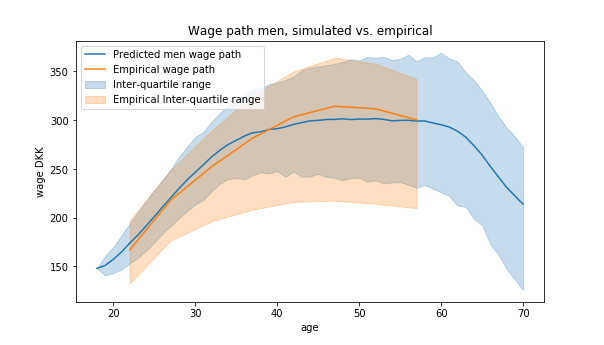
\includegraphics[width=1\linewidth]{figures/simulated_wage_path_variance_optimized_parameters_women.png}
  \caption{Men}
  \label{fig:sub1}
\end{subfigure}%
\begin{subfigure}{.5\textwidth}
  \centering
  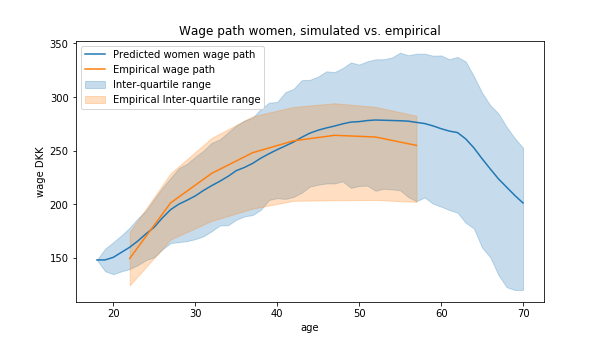
\includegraphics[width=1\linewidth]{figures/simulated_wage_path_variance_optimized_parameters_men.png}
  \caption{Women}
  \label{fig:sub2_wage_path}
\end{subfigure}
    \caption{Simulated Wage Process vs. Empirical Wage Process}
    \label{fig:sim_wage_vs_empirical_wage}
\end{figure}\label{sec:parameter_calibration}

Figure \ref{fig:sim_wage_vs_empirical_wage} compares the empirical wage process with the simulated. First looking to the \textit{wage path}, I conclude, that the Mincer equation seems to give a relatively good fit to the data even without taking education into account. The mean absolute error of the wage path of women is $10.61$ DKK, and for men the number is $5.84$ DKK, which considering the relatively simple parametric form of the process, is very good. Figure \ref{fig:sim_wage_vs_empirical_wage} also  show the empirical wage process is skewed. In this formulation of the mincer equation this is not possible. The width of the inter-quartile range seem to fit the wage path of men reasonably, but for women it slightly overshoots. I conclude the parameter values of the Mincer equation do seem to yield reasonable results, and they will be used throughout the paper. A side note about the empirical wage path of men and women is, that men do seem to experience a greater variance in their wage rates than women. Considering the work of both \textcite{francesconi_joint_2002} and \textcite{gayle_life-cyle_2006} that suggests that women on high income trajectories finds it less desirable to work, this is a puzzling result. The literature suggests that children could be one of the main drivers of heterogeneity observed in the wage rates of women, so when men have even higher wage rate differences, and these are not driven by children, one must conclude that other, probably equally important factors drive wage rate heterogeneity.



\section{Reinforcement Learning}
\label{sec:rl_theory}

\subsection{What is reinforcement learning}

Reinforcement learning is the study of "learning by interaction". As in the real world, when learning how to act, this is done by trial and error.

\subsection{The Environment/Agent interface}

The problem of learning by trial and error has a natural formulation by the environment/agent interface:

\begin{figure}
    \centering
    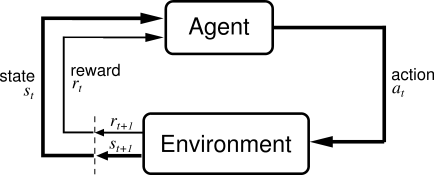
\includegraphics[scale=0.5]{figures/agent_environment_interface.png}
    \caption{Agent/Environment Interface}
    \label{fig:agent_enviroment_interface}
\end{figure}

The problem can be phrased the following way: An agent will over a series of discreet time steps $t=1, 2, \cdots, T$ take an action which will lead to some sort of reward (or in economic terms utility). So for each time step the agent gets information about the environments state $S_t$. The agent can then take an action $A_t$, which prompts the environment to return a reward $R_{t+1}$, and a new state $S_{t+1}$, which restarts the loop until the game terminates. The agents sole purpose is to maximize the cumulative rewards through out the game. It should be noted here that $R_t \in \R$. So the agent is optimizing over a sum of scalars. The representation of the state $S_t$ can be only partially observable in the reinforcment learning formulation. This game will lead to a trajectory of states, actions and rewards that look like:

\begin{equation}
    S_0, A_0, R_1, S_1, A_1, R_2, S_2, A_2, \cdots ,R_{T-1}, S_{T-1}, A_{T-1}, R_{T}
\end{equation}

However more formally certain assumption is necessary to perform any sort of modelling. The most fundamental assumption RL relies on is Markov Decision processes: A Markov decision process (MDP) can be described as:

\begin{equation}\label{eq:mdp1}
    p(s_t, r_t \mid s_{t-1},  a_{t-1}) = p(s_t, r_t \mid s_{t-1},\cdots, s_{0}, a_{t-1}, \cdots, a_{0}) = P(S_t = s_t, R_t = r_t \mid S_{t-1} = s_t, A_{t-1} = a_t)
\end{equation}

Breaking the equation \eqref{eq:mdp1} down we see that the MDP follows a true probability distribution. That is $R_t$ and $S_t$ is well defined probability distributions. More over another very important feature is that the probability distribution of $S_t$ and $R_t$ only depends on the last state and action. This turns out to be a very important assumptions to do any sort modelling. This implies that the state $s_t$ contains all relevant information about the past, which is what makes the problem a \textit{Markov} Decision Process. This condition/assumption yields certain important features. First, it implies that size of the probability distribution would not grow linearly as more and more states and actions was represented for the agent. Yielding the computations more and more expensive. Second thing which is important is, that allows for backward induction and dynamic programming (a topic which will be discussed later). Lastly this implies than when we model the system we must ensure that the state is represents all relevant information about the past.

From the equation \eqref{eq:mdp1} multiple statements can be derived, but most importantly one can derive, the expected rewards, which is what we is what the agent want to maximize:

\begin{equation}
    \E[R_t \mid A_{t-1} = a_{t-1}, S_{t-1} = {s_{t-1}}] = \int_{r_t} \int_{s_t} p(r_t, s_t \mid r_{t-1} s_{t-1}) d s_t d r_t 
\end{equation}

As mentioned in the start the agents goal is to maximize the cumulative rewards. This can be described as in equation:

\begin{equation}\label{eq:cum_rewards}
   G_t = R_{t+1}, R_{t+2}, R_{t+3}, \cdots R_{T}
\end{equation}

In general however the above formulation can be problematic with continuing tasks. That is if $T \rightarrow \infty$. Therefore discounting of rewards is usually implemented. Which have the nice economic implications, that agents in the real world tend to be impatient, and therefore more realistically real human agents:

\begin{equation}
    G_t = R_{t+1} + \gamma R_{t+2} + \gamma^2 R_{t+3} + \cdots = \sum_{k=0}^{T - t} \gamma^k R_{t+k+1}
\end{equation}

with $\gamma$ being the discount rate, yielding a geometric series, that is known to converge, if $R_k$ is bounded.

\subsection{Value function, Q-function, Policy function and the Bellman Equation}

To navigate in the environment usually a couple of things is considered: First the value-function:

\begin{equation}\label{eq:value_function1}
    v_{t}^{\pi}(s_t) = \E_t [G_t \mid S_t = s_t] = \E_t \lsp \sum_{k=0}^{T - t} \gamma^k R_{t+k+1} \bigg\vert S_t = s_t \rsp 
\end{equation}

Where it's implied in this formulation that the agent is following some policy $\pi$. A couple of things to note about \eqref{eq:value_function1}: Since the expectation is taken over a sum this is the same to take the sum over the expectations, yielding it possible to calculate the individual expected returns from following a policy, and using those to calculate the value function. Another formulation that lies close to the value-function is the Q-function which will be explored in this paper:

\begin{equation}
    q_t^{\pi} (s_t, a_t) = \E_t [G_t \mid S_t = s_t, A_t = a_t ] = \E_t \lsp \sum_{k=0}^{T - t} \gamma^k R_{t+k+1} \bigg\vert S_t = s_t, A_t = a_t\rsp 
\end{equation}

which only differ from the value function by also conditioning on the action, and not only the state. The value function and the Q-function shares the property that it maps the expected value of an state (or state action pair) to a scalar vale, where this value represent the cumulative, discounted rewards of following a certain policy. This has the nice property of allowing the agent to choose an action which maps to the highest expected value.

A policy function is a how the agent chooses its actions:

\begin{equation}
    \pi_t : \statespace \mapsto \actionspace 
\end{equation}

Some of the methods explored in this paper works by directly estimating the policy function, where as other works by estimating the value function or Q-function using these to find the correct optimal policy.

Using the expression of the value function we can now express the Bellman equation:

\begin{equation}
    v^{\pi}_{t} (s_t) = \E_t [G_t \mid S_t] = \E_t  \lsp R_{t+1} + \gamma G_{t+1} \mid S_t \rsp = \E_t \lsp R_{t+1} + \gamma v_{t+1}^{\pi}(s_{t+1}) \rsp
\end{equation}

A couple of things to note about the bellman equation: First and foremost one should consider that $\E [v_{t+1}^\pi(s_{t+1})]$ does not imply $v_{t+1}^{\pi}(\E[s_{t+1}])$, which has the consequence of considerable computational markup when solving a model using the Bellman Equation. Furthermore.

\subsection{Relationship to Dynamic Programming}\label{sec:dynamic_programming}

\textbf{BOOTSTRAP SKAL INTRODUCERES}

Dynamic programming, invented by Richard Bellman, allows for a way to find the optimal policy $\pi^{*}$ and the associated value function $v^{\pi^{*}}$ when following the optimal policy. To do dynamic programming, certain things are necessary. First the size of the statespace should be limited. That is due to the fact, that number of computations will increase exponentially with the number of states. Secondly it also requires that the entire MDP is known. So partially observable models f.x. cannot be used. In general it can be said that dynamic programming (and also reinforcement learning) is to use the value function to structure the search for good policies  \parencite{sutton_reinforcement_2018}. It's clear that if we have the optimal value function, we also have the optimal policy:

\begin{equation}
    v_t^{*}(s_t) = \underset{a_t}{\max} \lsp \E \lsp R_{t+1} + \gamma v^{*}_{t+1}(s_{t+1}) \mid S_t = s_t, A_t = a_t\rsp \rsp
\end{equation}

Dynamic programming problems can be solved by two different approaches: value function iteration and policy function iteration.

Policy function iteration consists of two steps: 1) an evaluation step. Which calculates the value of a policy, and 2) a policy improvement step.
Step 1 can be considered a prediction step, that by following a given policy calculates the associated value function for said policy. This is done by sweeping through the state space calculating the expected value of the state following the policy. This process continues until the algorithm has converged, where converged implies that the difference between the previous estimation of the value function and the current estimation of the value function, only differs below some threshold. The second step, policy improvement, follows the logic. Assume that the policy just used for the evaluation step is optimal. Then there should be no other strategy that would yield a higher value-function for all possible states. Now this can be written more formally as:

\begin{equation}
    \pi^*_t (s_t) \geq \tilde{\pi}(s_t)\qquad \forall s_t \in \statespace
\end{equation}

where $\tilde{\pi}$ is any arbitrary strategy. This also implies that if we at any point in the state space can find a policy that yields a higher value function than the current, then we should switch strategy. Which have now yielded a better strategy! If the during the sweep through state space, searching for better policies, a new policy is found. The process goes back to a policy evaluation step. This goes on until that there can be found no better policy than currently being employed. A graphical the process can be considered as shown in equation \eqref{eq:policyevaluation} where $\overset{\textbf{E}}{\longrightarrow}$ denotes a policy evaluation and $\overset{\textbf{I}}{\longrightarrow}$ denotes policy improvement:

\begin{equation}
    \label{eq:policyevaluation}
    \pi^0 \overset{\textbf{E}}{\longrightarrow}
    v^{\pi^0} \overset{\textbf{I}}{\longrightarrow} \pi^1 \overset{\textbf{E}}{\longrightarrow} v^{\pi^1} \overset{\textbf{I}}{\longrightarrow} \cdots \overset{\textbf{I}}{\longrightarrow} \pi^* \overset{\textbf{E}}{\longrightarrow} v^{\pi^*}
\end{equation}

The second approach value function computes a max over the value function implying only a single sweep through the state space in iteration of the loop, yielding it a much faster approach for solving the model. Value function iteration can be considered using the Bellman equation as an update rule. \parencite{sutton_reinforcement_2018}. The algorithm for value function iteration is described below:

\begin{algorithm}[H]
\SetAlgoLined
\KwResult{Yielding $\pi^*, v^*$}
 Algorithm parameter $\theta > 0$ determining accuracy of estimation\;
 Initialize $V(s)\quad \forall s \in \statespace$ except $V(terminal) = 0$\;
 \While{$\Delta > \theta$}{
    $\Delta \la 0$ \; 
    \ForEach{$s \in \statespace$}{
        $v \la V(s)$ \;
        $V(s) \la \underset{a}{\max} \E [R_{t+1}  + \gamma V(s') \mid A_t = a, S_t = s] $ \;
        $\Delta \la \max (\Delta, \mid  v - V(s) \mid )$
    }
 }
 \caption{Value Function Iteration}
\end{algorithm}

 So for each step sweep through the loop a single sweep through the state space is performed finding which action yields the highest associated value for a given state. Finally when the sweep is completed the associated policy evaluation can be done. Finding the value function. Again this algorithm terminates when the difference between the value function of the last sweep and the current value function is below some threshold.
 
 In economics very often a dynamic model will be solved using value function iteration but with the addition of using backwards induction. How is this possible. Just as the model presented in this paper. The model assumes an agent acting over $T$ time steps, terminating when the agent reaches a certain age. So in a sense the agent moves in a deterministic fashion towards the termination of the environment. This implies that one can solve such a model by only doing a single sweep through the state space! What will be done is that at the terminal period the agent will optimize his value function. Now using this value associated with the terminating period, the agent can consider his actions in $T-1$. Remembering that we can use the Bellman equation as an update step we can write:
 
 \begin{equation}
     V_{T-1}(s_{T-1}) = \underset{a_{T-1}}{\max}\E [R_{t+1} + \gamma V_T (s_T)]
 \end{equation}
 
 In other words, we can model all possible states that the agent can encounter in each time step of the model, making it possible to find the optimal value function $v^{\pi^*}$ and policy function $\pi^{*}$ by simple sweep through the state space using a combination of dynamic programming and backwards induction. The implementation of Value function iteration in this paper will be explored in a later section.
 
 \subsection{Overview of other Reinforcement learning techniques}.
 
Later in this paper I present three different reinforcement learning methods. Here i present some basic information that makes the reader able to digest the material presented. First it's important to address why not only use dynamic programming. Dynamic programming requires that a perfect model of the environment is accessible. This is due to the fact, that when calculating the expected value function for each action, the probability distribution of the reward and the next state, needs to formulated in an explicit form. The other techniques presented here does not have the same requirement. Secondly DP methods require that state space cannot be to large. The implementations presented later does not have the same requirements, allowing for approximating the value function and/or the policy function. Below i explain two different methods of learning \textit{Monte Carlo Methods} and \textit{Temporal Difference Learning} these being the two foundations of the reinforcement learning methods presented later.

\subsubsection{Monte Carlo Methods}

Before delving into MC-methods it is appropriate to introduce some more nomenclature: when talking about an \textit{episode} it should be understood as an agent moving through the environment from start to termination. When talking about a \textit{step} it should be understood as going from one state to the next in the environment. The best way to get a sense of Monte Carlo methods is to present the algorithm:

\begin{algorithm}[H]
\SetAlgoLined
\KwResult{Yielding $v^{\pi}$}
 Input: policy $\pi$ to be evaluated\;
 $Returns(s) \la$ an empty list $s \in \statespace$\; 
 \While{Forever}{
    Generate an episode: $S_0, A_0, R_1, S_1, A_1, \cdots S_{T-1}, A_{t-1}, R_T$\; 
    $G \la 0$ \;
    \ForEach{step in episode, $t = \{T -1 , T-2 , \cdots, 0\}$}{
        $G \la \gamma G + R_{t+1}$\;
        \If{$S_t \notin \{S_{t-1}, S_{t-2}, \cdots S_0 \}$}{
            Append $G$ to $Returns(S_t)$ \;
            $V(S_t) \la average(Returns(S_t))$ \;
        }
    }
 }
 \caption{First-Visit MC prediction, for estimating $v^{\pi}$}
 \label{alg:mcfirstvisit}
\end{algorithm}

Algorithm \ref{alg:mcfirstvisit} shows how the general concept of estimating the value function for given policy. Things to be noted: First and foremost the algorithm presented above is made to a tabular case, i.e discrete state space. This will be dealt with in the algorithm presented later in this paper. Second it is assumed that the policy stays constant. That is, the policy does not update as more and more episodes are experience, which defeats the purpose of learning how to interact with the environment. Addressing the latter part usually the policy is updated, and the you could discard the old experience. However another possibility is to accept the non stationarity of the data collected, and update the policy using the data from a previous policy, hoping that with time the algorithm will converge.

Consider now how to do Monte Carlo Control, i.e. approximating the optimal policy. Just as with policy iteration the pattern followed is:

\begin{equation}
    \label{eq:montecarlocontrol}
    \pi^0 \overset{\textbf{E}}{\longrightarrow}
    q^{\pi^0} \overset{\textbf{I}}{\longrightarrow} \pi^1 \overset{\textbf{E}}{\longrightarrow} q^{\pi^1} \overset{\textbf{I}}{\longrightarrow} \cdots \overset{\textbf{I}}{\longrightarrow} \pi^* \overset{\textbf{E}}{\longrightarrow} q^{\pi^*}
\end{equation}

Just with the caveat that instead of considering the value function, the Q-function (state-action pair) is used for policy evaluation. Policy improvement is done by making the policy greedy with respect to the current estimated Q-function \parencite{sutton_reinforcement_2018}. Since the Q-function instead of the value function is used, no model us needed to construct a greedy policy \parencite{sutton_reinforcement_2018}. The greedy policy is the one that for each $s \in \statespace$ deterministically chooses an action with maximal action-value:

\begin{equation}
    \pi(S_t) = \underset{a}{\argmax}  Q( S_t, a )
\end{equation}

Now this algorithm is made under the assumption of \textit{exploring starts} and under the assumption of \textit{infinite epsiodes}. The assumption of inifinte episodes is to ensure convergence, and in practice the algorithm is usually run until the algorithm has converged by some high number of episodes. The more problematic assumption is that of exploring starts. This is due to the fact, that in reality we would not assume that there is a uniform distribution of starting in all states $s \in \statespace$, and proceed the episode from that starting point. This is an essential assumption, because otherwise, one could not know the value function of unexplored states without visiting them. This leads to the concept of on-policy control. On policy control is most often implemented using an $\epsilon$-greedy strategy. The implication is that $P(A=a \mid S=s, q^{\pi}) > 0, \forall a \in \actionspace, s \in \statespace$. Where the non optimal action is choosen by drawing from an uniform distribution over all actions with probability $\epsilon$. Off-policy control works by having two different policies one which works by doing the optimal action (target policy $\pi$), and a second policy that moves to investigate the state space (behavior policy $b$). Using the experience from these two policies importance sampling can be used to estimate the value function! It's required that the behavior policy has a non zero probability to any action for any state.

\subsubsection{Temporal Difference Learning}

Temporal Difference (TD) learning is a combination of ideas taken from Dynamic Programming and Monte Carlo Methods. It takes from Monte Carlo methods, that you do not need a perfect model of the environment. It takes from Dynamic Programming the bootstrapping, i.e. it uses learned estimates to update, without needing the final outcome. Just as Monte Carlo methods, Temporal difference methods has a prediction and control element. 

TD prediction can be summarized in the equation:

\begin{equation}
    V(S_t) \leftarrow V(S_t) + \alpha \lsp R_{t+1} + \gamma V(S_{t+1}) - V(S_t) \rsp
\end{equation}

The equation states that $V(S_t)$ should be updated according to the return in a given period + the value function of the next period $V(S_{t+1})$. This method is called TD(0), since it only uses 1 step to update the value function. In essence TD methods learn a guess from a guess. This allows for not having a complete model of the environment (of rewards and next-state probability distributions). Compared to MC methods the TD learning can learn at each step - update it's estimate at each point in time. It is also proven, that for any policy $\pi$ kept fixed, then a TD(0) algorithm will converge to $v^{\pi}$ \parencite{sutton_reinforcement_2018}. Even though, an open mathematical question, in practice it is found that TD methods converge faster than MC methods \parencite{sutton_reinforcement_2018}.

Control with temporal difference learning, can also be separated into on-policy control and off-policy control. The most used on-policy control for TD methods is called SARSA (state, action, reward, state, action). Just as with MC methods a need to trade off exploitation and exploration is present. The agent want to see new parts of the state space (exploration), but should also use (exploit) what is assumed to be the optimal choice given the value function associated with the current value function. In this case instead of using the value function instead, consider the case of using the state-action pair function $Q(S_t, A_t)$, yielding the update rule:

\begin{equation}
    Q(S_t, A_t) \leftarrow Q(S_t, A_t) + \alpha \lsp R_{t+1} + \gamma Q(S_{t+1}, A_{t+1}) - Q(S_t, A_t) \rsp
\end{equation}

This update is made after each step in a non-terminal state of the environment. As in on-policy methods $q^{\pi}$ is estimated for the policy $\pi$ whilst at the same time greedy updating $\pi$ with respect to $q^{pi}$. Exploration can again be done using an epsilon greedy approach.

Off-policy control can be done by using Q-learning. Q-learning has the slight twist on update the rule for SARSA that:

\begin{equation}
    Q(S_t, A_t) \leftarrow Q(S_t, A_t) + \alpha \lsp R_{t+1} + \gamma \underset{a}{\max} Q(S_{t + 1}, a) - Q(S_t, A_t) \rsp 
\end{equation}

Actions is still chosen by an $\epsilon$-greedy policy, the difference here being the updating rule presenting a different policy than the actual policy, since we assume that we greedily chooses the action in time $t+1$ conditional on the state. Q-learning and double Q-learning will be explored in depth later when describing the algorithms used in this paper.

\subsection{Landmarks}

Finally, before moving a brief overview of environments/games where reinforcement learning have been instrumental. The first big success of reinforcement learning was made by Tesauro in 1992 creating an agent of learning to play backgammon trough self play. Using an artificial neural network to approximate the value function, and using a temporal difference algorithm, the algorithm was capable of playing expert level backgammon. In 2011 the IBM Watson algorithm won in jeopardy using the same methods as Tesauro for his backgammon agent. In 2013 the company DeepMind (now acquired by google), showed that it was possible for a reinforcement learning algorithm to learn to play video games. Here an important feat was, that it was fed the raw image input and used an artificial neural network to transform this image into an representation of the state space allowing for learning how to navigate in the environment. In 2016 DeepMind created AlphaGo and a year later AlphaGo Zero, which learned to master the game of Go. This was assumed in a long time to be a hard problem for learning algorithm due to its very large state and action space. The first iteration used expert players to learn the game, while the AlphaGo zero used only selfplay. These examples show that the feasibility of these algorithms to learn to navigate in complicated environments, might leave a way for high dimensional dynamic economic models to be solved using reinforcement learning methods.

\section{Deep Learning}
\label{sec:deep_learning}


\subsection{Why machine learning}

Machine learning methods try to model either the joint or the marginal distribution of some covariates and some target. In statistics a model is usually explicitly formulated. A typical example could be linear regression. The covariates is decided on, and transformed such that they fit the desired model. The linear regression will yield a parameter vector which can then be interpreted. And this interpretation is usually the focus - parameter inference. Example: Does an increase in the minimum salary have a negative effect on BNP pr. capita. Machine Learning focuses on prediction. That is, the objective is to predict some target conditional on some covariates. The specific model is not necessarily important. Instead a focus on Out-Of-Sample error is the focus. These predictive methods lend themselves well where causal inference is not needed. Example: What is the expected consumption on a monthly basis by person with a given set of characteristics. When formulating a traditional econometric method, f.x. OLS, there is standard ways to infer if the model is well specified. In machine learning, in general the same asymptotic results regarding regularization of the model is not possible. Usually sample splitting will be used instead. Take a data set, split the data set into two partitions a test set and a training set. First the hyper parameters of the machine learning algorithm is tuned, usually by finding which set of hyper parameters that yield the best performance on the training data. Usually a cross validation procedure is used to find this. The final algorithm is only used on the test data set once yielding the out-of-sample performance. Machine learning methods, as mentioned before usually has associated hyper parameters. These are parameters of the model, which is not fitted by training the data, rather these are specifications of the algorithm before  training the model. Much of machine learning is about finding the right hyper parameters and regularizing the model in an intelligent way \parencite{friedman_elements_2001}. Now why is this paper concerned with ML methods? This is due to the fact, that when estimating the value function, or the policy function, one cannot be sure that this follows a linear function. In fact value functions and policy functions might be highly non-linear, which is where machine learning methods shine. Furthermore what is modelled trying to capture the value function is a conditional expectation: $ \E[Y \mid X=x]$, which can be directly translated into the expected value function for a given state. In this case the causal interpretation of the influence of a specific state on the value function is not of interest, rather it's the accuracy of the expected value function\footnote{Obviously, intelligent agents usually do causal inference on their actions. They might not do a certain action exactly because they have some causal notion of how the environment will evolve conditional on their action.}. Usually deep neural networks has been the usual way to implement reinforcement algorithms, however other machine learning methods can also be used. Deep Learning methods has though they convenient property of online updating of it's weights. In other words, as more data comes in, the neural network can be incrementally fitted to the new data.

\subsection{Deep Neural Networks}

Deep learning (feed forward networks) which is used in this paper is in fact just layered non-linear functions. Figure \ref{fig:feedforwardnetwork} illustrates the architechture of a deep neural network \footnote{Figure found at \url{https://upload.wikimedia.org/wikipedia/commons/thumb/c/c2/MultiLayerNeuralNetworkBigger_english.png/381px-MultiLayerNeuralNetworkBigger_english.png}}.

\begin{figure}[ht]
    \centering
    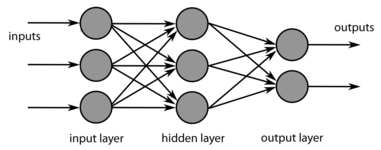
\includegraphics[scale=0.6]{figures/feedforwardnetworkillustration.png}
    \caption{Illustration of feed forward neural network. }
    \label{fig:feedforwardnetwork}
\end{figure}

The network can be described as having an \textit{input layer}, that takes the covariates, $\textbf{x}$. The \textit{hidden layer} makes a transformation, of the previous layer, that also implies that a hidden layer, can be followed by an arbitrary number of other hidden layers. Lastly and \textit{output layer} that maps the representation of the hidden layer into the desired output. For classification that might be a one-hot encoding of the classes, and for regression it might to a single real valued scalar.

As illustrated in figure \ref{fig:feedforwardnetwork}, each layers is broken down into smaller cells. The number of cells in each layer corresponds to the width of the layer. The wider the layer the more flexible representation the given layer is capable of doing. The hidden cells work as mentioned by creating a non-linear transformation of the input from last layer:

\begin{equation}
    z_i^{+} = g(\textbf{z}; \theta) = g(\textbf{w}^T \cdot \textbf{z} + b)
\end{equation}

The output of cell \textit{i} is the real valued scaler $z_i^+$. $g$ is the activation function that maps the input into the output. $\textbf{w}$ is the weights of dot product, $\textbf{z}$ is a vector of the outputs from the last layer, and $b$ is bias or the constant in the activation. In that sense the activation looks like a linear regression squashed through an activation function $g$. Multiple different activations functions has been proposed. Originally the logistic function was prefered, but in later years the rectified linear unit activation function has been popular \parencite{goodfellow_deep_2016}:

\begin{equation}
    \textbf{Rectified Linear Unit: }  \max \lcp 0, \textbf{w}^T \cdot \textbf{z} + b \rcp
\end{equation}

The neural network can in other words be considered a function $f$, that takes an input $\textbf{x}$ and maps it to some output $y$, parametrized by $\theta$, which is a collection of all the weights and biases associated with each individual cell.

\subsection{Stochastic Gradient Descent and Optimization}

The neural network is estimated (or trained) by using stochastic gradient descent. This is possible due to the fact, that the networks can be represented as set of nested functions, such that the chain rule can be applied. The loss function can in other words be differentiated with respect to the parameter vector $\theta$ as shown below:

\begin{equation}\label{eq:loss_function}
    \frac{\partial}{\partial\theta} \Loss (\textbf{X}, \textbf{Y}, \theta) = \frac{\partial}{\partial\theta} \lp \sum \ell_i \rp = \frac{\partial}{\partial\theta} \lp \sum \lp \hat{Y}_i  - Y_i \rp^2 \rp = \frac{\partial}{\partial\theta} \lp \sum \lp f^{\theta}(X_i)  - Y_i \rp^2 \rp
\end{equation}

In equation \eqref{eq:loss_function} the loss function $\Loss$ is assumed be be a mean squared error, in other words a regression problem. The optimization works by minimizing the loss with respect to the parameters $\theta$. In modern neural network architectures it is not unusual that such network has in the excess of a million parameters. Furthermore the objective function of the optimization cannot be assumed to be convex. This implies that analytical solutions for solving deep neural networks is infeasible. Instead gradient descent is used for estimating the parameters of the network. The update rule of the parameters can be described as \parencite{goodfellow_deep_2016}:

\begin{equation}
    \theta \la \theta - \alpha \nabla_{\theta} \Loss(\textbf{X}, \textbf{Y}, \theta)
\end{equation}

So for each step in the algorithm the derivative with of the loss function with respect to the parameters can be calculated, and the parameters can be updated by taking a small step of size $\alpha$ in the direction in parameter space that reduces the loss. Stochastic gradient is a response to the fact that it can be computationally expensive to calculate the gradient for the entire data set in each update step. This is important for deep neural networks, since the training period of a large network, even on optimized hardware, can take a very long time, so any speed up for the training is important. In practice this implies that the training data is split into mini batches usually of size 32 to 128. The optimization is then performed on each of the small batches, taking a small step of size $\alpha$ for each step.




\section{Soution methods}\label{sec:solution_methods}

\subsection{Value Function Iteration}

In this section 3 different solution methods i presented. I lead with modification of value function iteration, next deep Q-Learning is presented ending with double deep Q-learning iteration.

The value function iteration presented in this paper has certain modifications to the algorithm presented in \ref{sec:dynamic_programming}. First and foremost, I consider the Q-function instead of the value function, allowing to store state-action value pairs. Second it should be noted that in this formulation some of the states are continuous, not allowing for tabular solutions. Thirdly, the dimension of the state-space + the size of the grid made it infeasible\footnote{In my initial attempt to solve the model by value function iteration, I attempted to get the expectation of the value function using Gauss-Hermite integration, and discretizing the state space. The solution time was infeasible, which was why my approach changed.} to solve the model by classical ways of solving a model using backwards induction an discretizing the state space. 

The model is solved using backwards induction. This is due to the fact the model terminates in a deterministic fashion when the agents reaches a certain age. For each step a large random sample of states is drawn conditioning on a given age. For each of the states the agent takes each of the possible actions storing the results. This way a large sample of rewards and states can be generated. Furthermore for each action taken (if the state is not terminal) the  Q-function can be evaluated in the new state, taken the max of each possible action, allowing for the estimation of the value function. A graphical representation of the concept is shown in figure \ref{fig:vfi_figure}. 

\begin{figure}[ht]
    \centering
    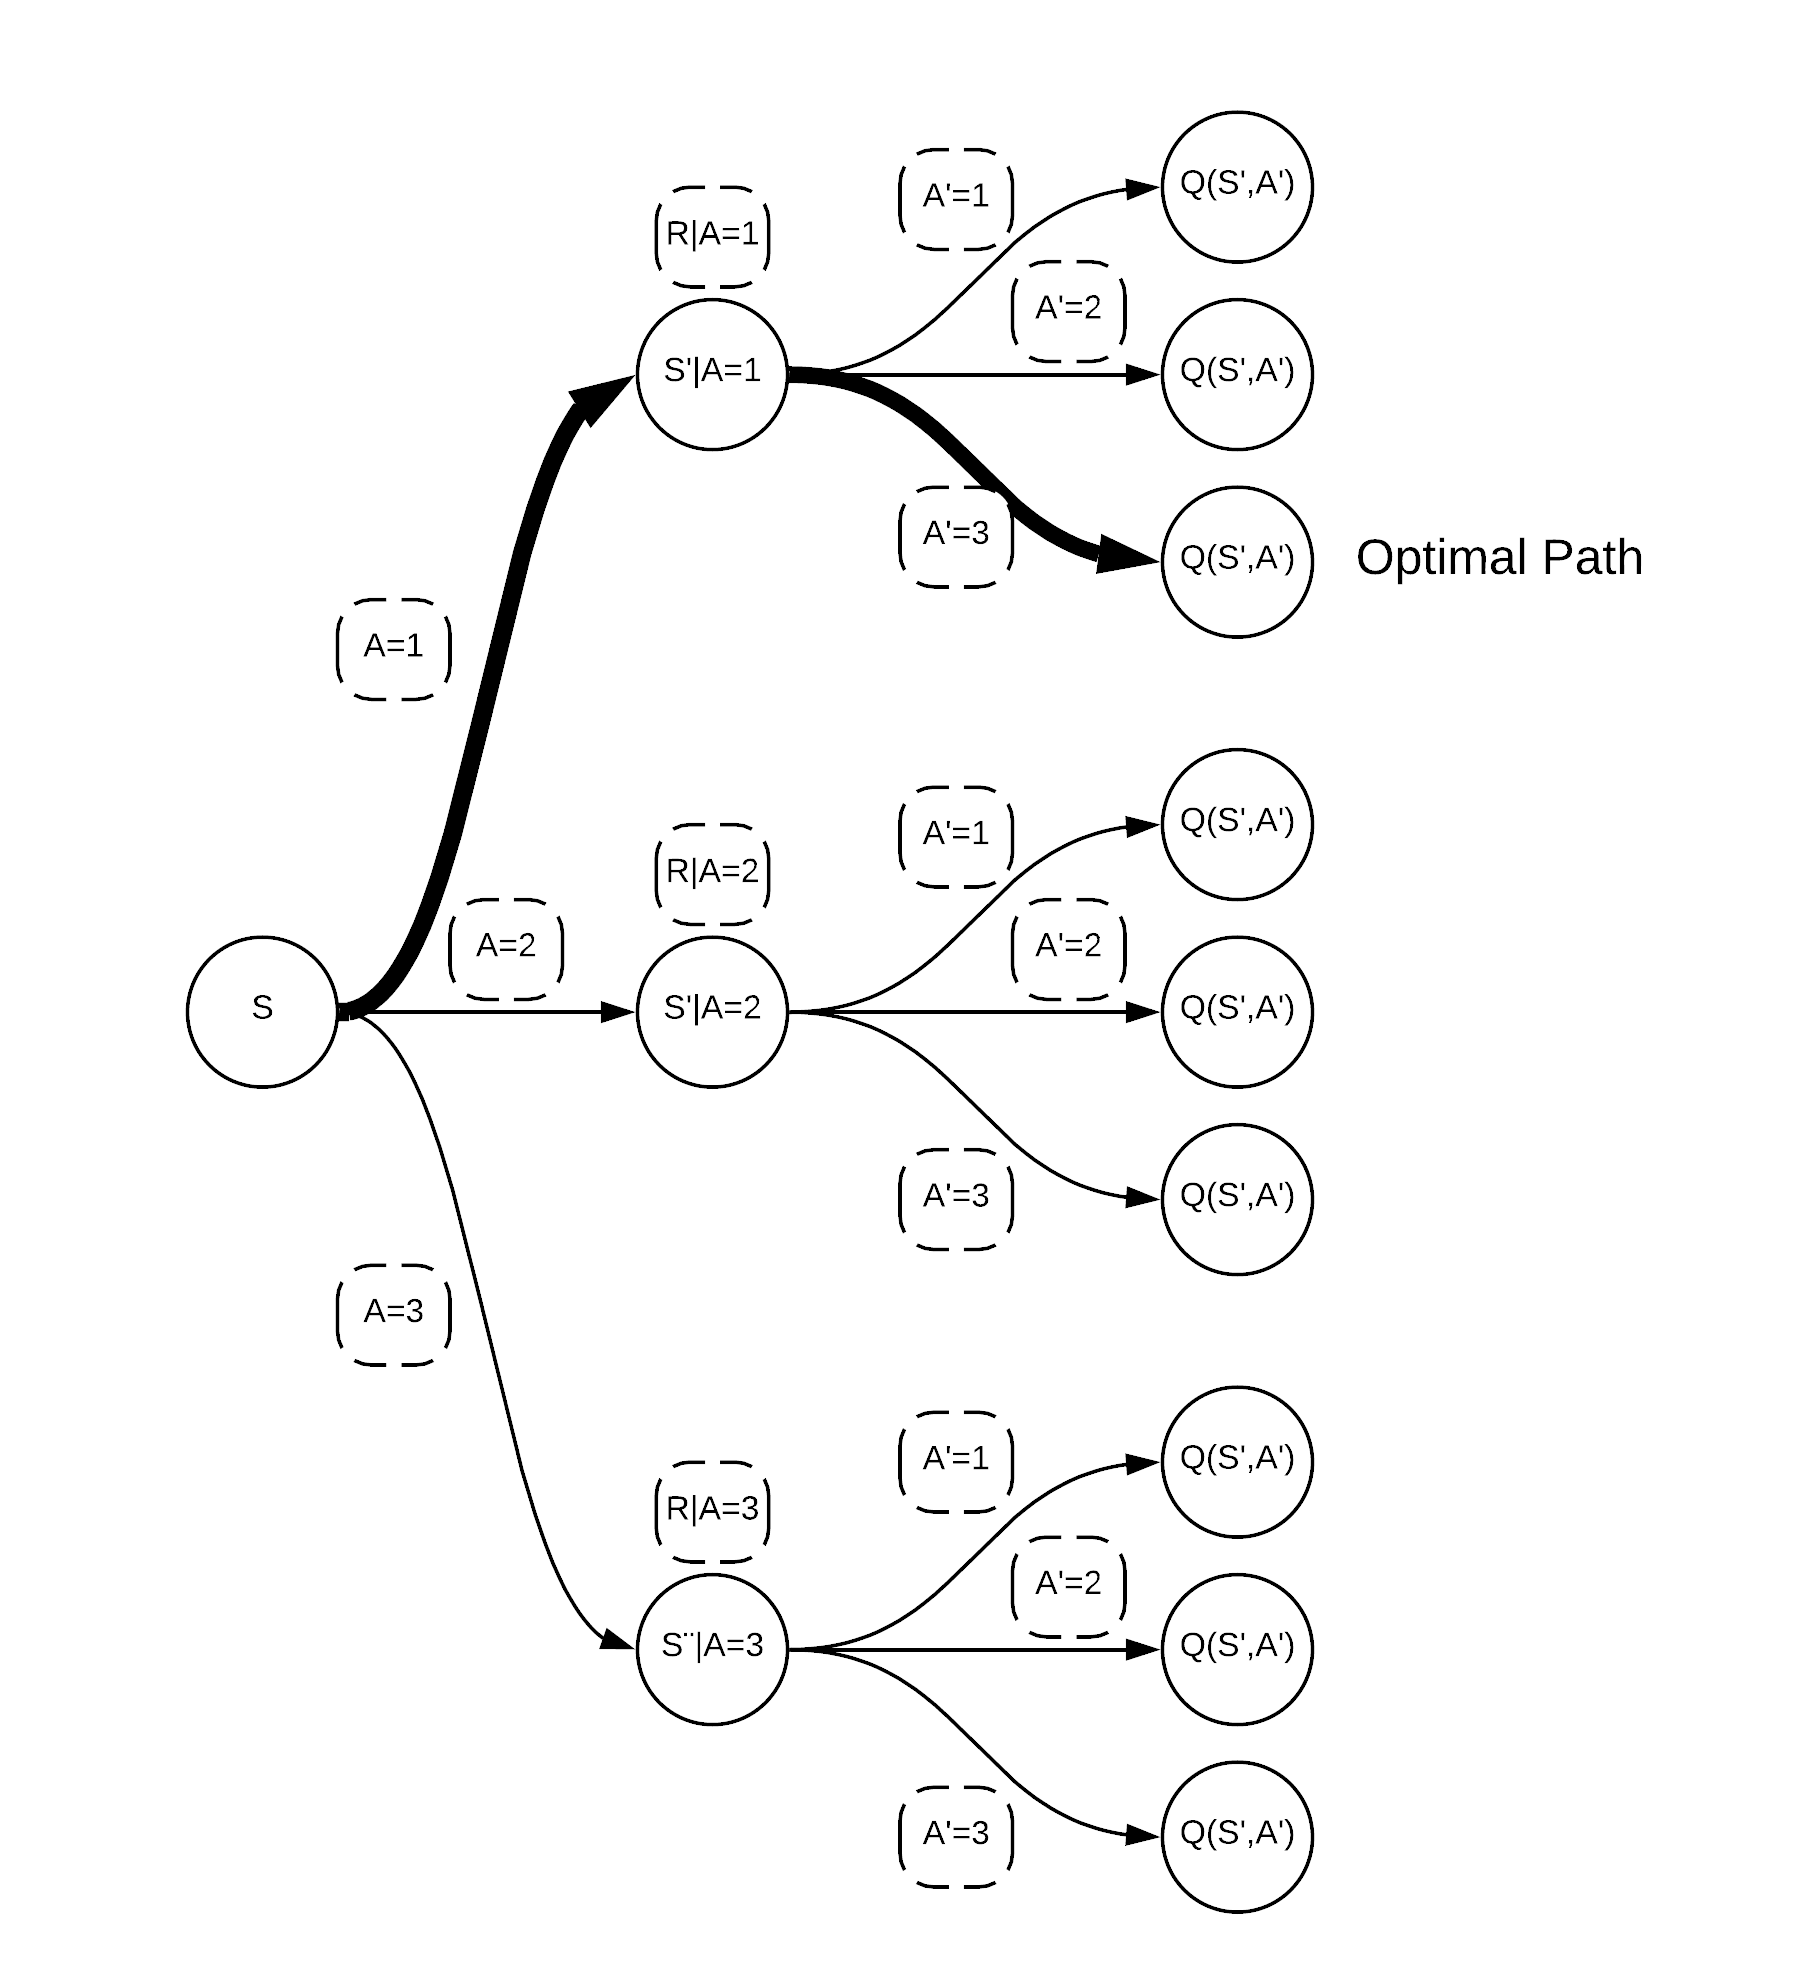
\includegraphics[scale=0.15]{figures/vfi_figure.png}
    \caption{Value function iteration using Q-function}
    \label{fig:vfi_figure}
\end{figure}

The Q-function for each action in the actionspace is made by mapping each $a\in \actionspace$:

\begin{equation}
 Q(S_t, A_t=a) = R_t + \gamma \underset{a_{t+1}\in \actionspace}{\max} Q(S_{t+1}, a_{t+1})
\end{equation}

In that sense this can be considered akin to Monte Carlo integration, however instead of approximating the expectation in a single point, rather find the distribution of the rewards + discounted value function over the entire state space. The idea is to approximate the integral by using a statistical method, in this case Deep Learning even though another machine learning method would be equally good. Consider $f$ to be a deep neural network, that has the property:

\begin{equation}
    f: \statespace \mapsto\R^{\mid \actionspace \mid}
\end{equation}

For a given point in state space a prediction of the value function is computed for each possible action. This implies the method only is feasible for discrete state space. By trying to reduce the mean squared error between the the true values of the Q-function, and the prediction, the $\E[Q(a, s)]$ can be found, which corresponds to integration as could be done using Gauss Hermite or Monte Carlo integration. The algorithm is presented in algorithm \ref{alg:dqi}.

\begin{algorithm}[H]
\SetAlgoLined
\KwResult{Estimated Q function}
 Initialize $\tilde{Age} = Age_{max}$\;
 Initialize empty lists for storing results: $X, Y$\;
 Initialize memory counter $j=1$\;
 \While{$\tilde{Age} > Age_{min}$}{
  Draw $\{s_{i}\}_{i=1}^{N}$, where $s_i \sim Uniform(\statespace) \mid Age=\tilde{Age}$ \;
  \ForEach{$s_{i}$}{
  Create empty array $Z$ of length $\mid \actionspace \mid$\;
  \eIf{$\tilde{Age}= Age_{max}$}{
   \ForEach{$a_k \in \actionspace$}{
    $Z[k] \leftarrow R_{t+1}, \quad  R_{t+1}\sim \mathcal{E}\mid A_t = a_k, S_t = s_{i}$ \;
   }
   }{
   \ForEach{$a_k \in \actionspace$}{
    $Z[k] \leftarrow R_{t+1} + \gamma \underset{a \in \actionspace}{\max} \hat{Q}(S_{t+1}, a), \quad  R_{t+1}, S_{t+1} \sim \mathcal{E} \mid A_t = a_k, S_t = s_{i} $\;
    }
  }
  $Y[j] \leftarrow Z, X[j] \leftarrow s_i$\;
  $j = j + 1$\;
  }
  Estimate $\hat{Q}$ by training a Deep NN using samples from $X, Y$\;
  Decrease $\tilde{Age}$ be one\;
 }
 \caption{Deep Q-function iteration solution method}
 \label{alg:dqi}
 \end{algorithm}

Since i use a deep neural network to approximate the $Q$-function, the architecture and hyper parameters of the network needs to be considered. The same is true for the sampling scheme.

For each age i draw 20.000 random samples. This is because any smaller number of draw seemed to be detrimental to the performance. This is inline with standard Deep Learning practices. These kinds of network is known to be very data hungry. When training the network i draw a random sample of 100.000 observations. If I have not yet accumulated 100.000 observations the algorithm draws all observations. The architecture of network is fairly simple being a two-layer fully connected network. First layer being 16 nodes wide, second fully connected layer being 8 nodes wide. I found that mini batching, did not seem to work well on this particular task, and instead i train on all observations, using a validation split of 30 \%, training for a maximum of 150 epochs\footnote{A epoch corresponds to a full sweep through the the data set.} and finally i allow for early stopping, that is, when the validation loss is not furthering decreasing i stop the training of the network. I do allow the algorithm a patience of 5. Implying that the algorithm will try to lower its validation loss for five additional epochs before terminating the training.


\begin{figure}[ht]
\begin{subfigure}{.5\textwidth}
  \centering
  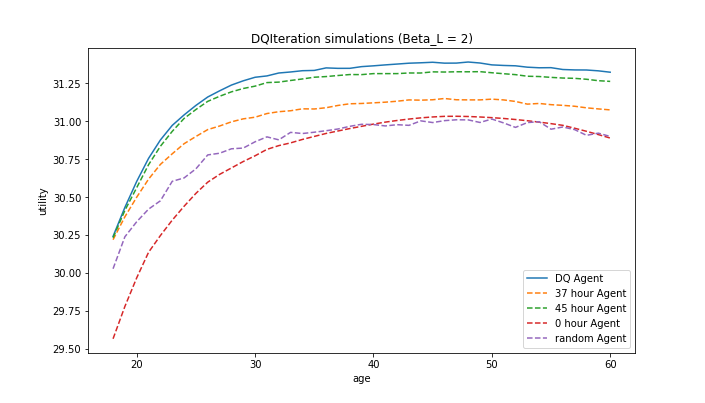
\includegraphics[width=1\linewidth]{figures/dqi_model1_beta_2_solution_benchmark_paths.png}
  \caption{Simulated Paths}
  \label{fig:dqi_solution_beta2_path}
\end{subfigure}%
\begin{subfigure}{.5\textwidth}
  \centering
  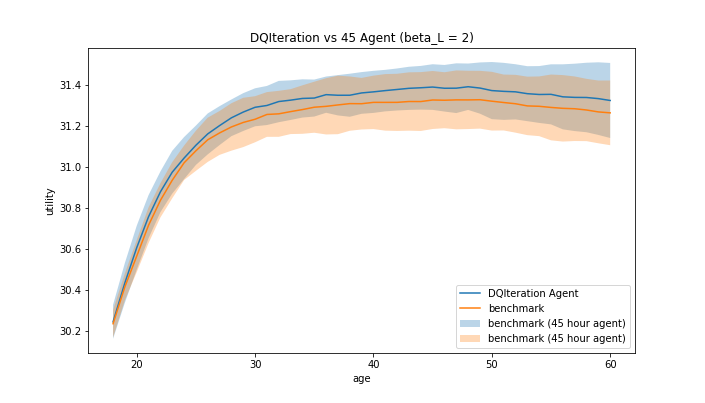
\includegraphics[width=1\linewidth]{figures/dqi_model1_beta_2_solution_benchmark_variance.png}
  \caption{Variance of Paths}
  \label{fig:dqi_solution_beta2_var}
\end{subfigure}
    \caption{Value Function Iteration solution vs. benchmark $(\beta_L = 2)$}
    \label{fig:dqi_solution_beta2}
\end{figure}

\begin{figure}[ht]
\begin{subfigure}{.5\textwidth}
  \centering
  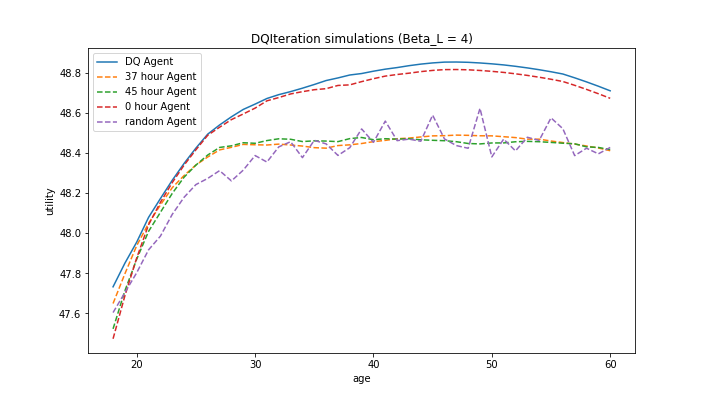
\includegraphics[width=1\linewidth]{figures/dqi_model1_beta_4_solution_benchmark_paths.png}
  \caption{Simulated Paths}
  \label{fig:dqi_solution_beta4_path}
\end{subfigure}%
\begin{subfigure}{.5\textwidth}
  \centering
  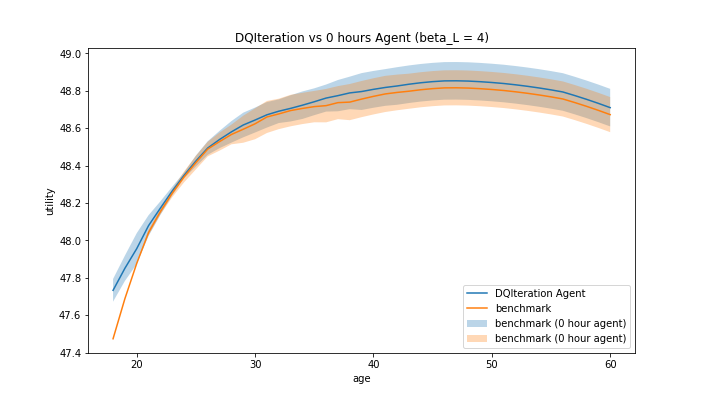
\includegraphics[width=1\linewidth]{figures/dqi_model1_beta_4_solution_benchmark_variance.png}
  \caption{Variance of Paths}
  \label{fig:dqi_solution_beta4_var}
\end{subfigure}
    \caption{Value Function Iteration solution vs. benchmark $(\beta_L = 4)$}
    \label{fig:dqi_solution_beta4}
\end{figure}

Figure \ref{fig:dqi_solution_beta2} and \ref{fig:dqi_solution_beta4} shows the results of the Value Function Iteration algorithm\footnote{The plots use the name DQIteration (Deep Q-Function Iteration) instead of Value Function Iteration.} compared to 4 benchmarks. Three deterministic agents working either $0$, $37$ or $45$ hours pr. week and one agent taking random actions. Figure \ref{fig:dqi_solution_beta2} shows the utility for each step over the life cycle when the preference for leisure is fixed at $\beta_L = 2$. As the figure shows the VFI agent learns to navigate the environment, just as well as the best deterministic agent. Looking to the right hand side plot of \ref{fig:dqi_solution_beta2} it is clear that there is a great overlap between the two agents. The variance of the path is represented as one standard deviation of the utility for a given age for all episodes of the given agent. Figure \ref{fig:dqi_solution_beta4} compares the benchmark agents with the VFI solution when considering a preference for leisure $\beta_L = 4$. Again the VFI solution is as good as the best benchmark.

\subsection{Deep Q-learning}

In this paper I implement\footnote{Originally I used my own implementation, however slow performance, caused me to use another implementation allowing for a speed up of a factor of 10. The same is true for the Double Deep Q-learning algorithm.} the deep Q-learning algorithm used by \textcite{mnih_playing_2013} for beating Atari games as a way to solve model. A few modifications is made to the original implementation, due to the fact, the environment they were navigating only returned sensory data (an RGB representation of an image), where a part of the their achievement was to transform these images into features that which the value function accurately could map into scores of the game. Another difference is that this paper implements a scaling module of the variables for better performance.

Just as described in section \ref{sec:rl_theory} the algorithm tries to maximize the Bellman equation. However now the value-function is estimated using Deep neural network as a function approximator. Mathematically this can be described as finding:

\begin{equation}
    Q^*(S_t,A_t) = \E [R_{t+1} + \underset{a}{\max}  Q^*(S_{t+1}, a) \mid S_t, A_t]
\end{equation}

However here $Q^*(S, A)$ is approximated by a parametric function (in this case a Deep Neural Network) $Q(S, A ; \theta)$. Following the terminology of \textcite{mnih_playing_2013}, this function approximator is referred to as the Q-network. The Q-network can be trained using stochastic gradient descent as described in section \ref{sec:deep_learning}:

\begin{equation}
    \Loss_i(\theta_i) = \E \lsp (Y_i - Q(S_t, A_t ; \theta_i))^2 \rsp
\end{equation}

where:

\begin{equation}
    Y_i = \E [R_{t+1} + \gamma \underset{a}\max Q(S_{t+1}, a; \theta_{i-1}) \mid S_t, A_t ]
\end{equation}

where $i$ implies the iteration of the algorithm, such $i$ increments by one for each update of the parameters $\theta$. This implies the update equation determining the update:

\begin{equation}
    \nabla_{\theta_i} \Loss_i (\theta_i)  \E \lsp \lp Y_i - Q(S_t, A_t ; \theta) \rp \nabla_{\theta_i} Q(S_t, A_t; \theta_i) \rsp
\end{equation}

Where i follow the formulation of \textcite{mnih_playing_2013} that $Q(S_{t+1}, A_{t+1}; \theta_{i-1})$ is held fixed, allowing for just writing $Y_i$, and not the parametric form of $Y_i$.

A traditional choice would be to update the weight after each step in the algorithm only using the last sample. This would the correspond to the traditional Q-learning algorithm. This was the approach used in by to create the TD Gammon created by Tesauro\footnote{I have not been able to get access to the original paper, so I have relied on the description made by Sutton and Barto.} as described by \textcite{sutton_reinforcement_2018}. This approach of using Q-learning with a non-linear function approximator has been shown to diverge under certain circumstances, and did not extend itself well to learning any other game than backgammon \textcite{tsitsiklis_analysis_1997}. To accommodate this problem a replay buffer is implemented. At each step a entry is made to the replay memory containing $(s_t, a_t, r_t, s_{t+1})$. This data set $\mathcal{D}$ has a capacity of $N$ entries. Using the replay memory a random mini batch is sampled used to update the weights of the Q-network. Note here that the capacity of the memory buffer should be greater, by a substantial margin than the number of samples drawn. The random sample has a couple of advantages. It decorrelate the observations used to update the weights, allowing for better training \textcite{mnih_playing_2013}. Using a replay buffer requires off-policy learning which is the reason for using Q-learning. This is due to the fact, that current parameters $\theta$ is not the same as those generating the data. Note that experiences is drawn randomly, and no experiences (which could have important insights) is prioritized. The full algorithm is summarized in algorithm \ref{alg:dqlearning}.

\begin{algorithm}[H]
\SetAlgoLined
 Initialize replay memory $\mathcal{D}$ with capacity $N$\;
 Initialize action-value function $Q$ with random weights\;
 Initialize memory counter $j=1$\;
 \ForEach {episode $\in \{1, 2, \cdots M \}$}{
  Initialize sequence with an initial state $s_1$. This is drawn randomly.\;
    \For{$t \in \{1, 2, \cdots, T \}$}{
    With probability $\epsilon$ select a random action $a_t$\;
    Otherwise select $A_t = \underset{a}{\argmax}Q^*(S_t, a ; \theta)$\;
    Execute action $A_t$ in environment and observe reward $R_t$ and the new state $S_{t+1}$\;
    Store transition $(S_t, A_t, R_{t+1}, S_{t+1})$ in $\mathcal{D}$\;
    Sample random mini-batch of transitions $(S_t, A_t, R_{t+1}, S_{t+1})$ from $\mathcal{D}$\;
    Set $
      Y_j = \begin{cases}
        R_j & \text{if terminal states} \\
        R_j + \gamma \underset{a}{\max}Q(S_{t+1}, a; \theta) & \text{if non-terminal states}
      \end{cases}
    $ \;
    Perform gradient descent step on $(Y_j - Q(S_t, A_t ; \theta))^2$ \;
    Increment $j$\;
  }
}
\caption{Deep Q-learning}
\label{alg:dqlearning}
\end{algorithm}

Following the implementation \textcite{mnih_playing_2013} a trick is applied to reduce the number of computations needed when running the algorithm. Ordinarily the Q-function maps a state action pair to a scalar value estimate of the value function. The most obvious implementation would let the action be part of the input to the function, however, such implementation would require $\mid \actionspace \mid$ number of look ups, at each step. This is due to the fact that each action in the action space must be used for evaluation. Instead the Q-function in this implementation maps the state space to a scalar value for each action, just as described in section \ref{sec:rl_theory}: $Q: \statespace \mapsto \R^{\mid \actionspace \mid}$. 

The solution used the following hyper parameters and architecture decisions: The Deep Neural network consists of an input layer of same size as the state space, followed by two fully connected layers of width $256$ using rectified linear units as activation functions. Finally the network uses a linear output layer for its predictions. The output layer is of the same size as the action space. The learning rate, $\alpha=0.0005$ and I let epsilon be decremented after each update by: $\epsilon_i = \max (\epsilon_{i-1} \cdot 0.9999, 0.01$), where $0.01$ is the minimum exploration that can be done. The replay buffer has a capacity of 1 million rows, and the mini batches used for updating the parameters is $64$ rows. I scale the state space so that each variable approximately has mean zero and standard deviation of 1 when doing the batch training. \textcite{goodfellow_deep_2016} argues that it increases performance, and in general accepted as being an important step for getting good performance out of neural networks . The impatience parameter is set to $\gamma=0.99$, using a standard value. I make the parameter $\beta_L$ a part of the state space, drawing a random value (uniformly) in the interval $[0.2, 6.0]$ at the beginning of each episode, letting the agent navigate through the environment with given preference for leisure. This is done, so only a single solution of the model is necessary for estimating the parameter later. I scale the rewards (so they are approximate zero mean and have a standard deviation of 1, conditional on the $\beta_L$ value. Again this is done to improve the training performance and to do introspection; it becomes possible to see if there is any trend in the training performance. The algorithm is trained for 3000 episodes. Figure \ref{fig:training_performance_simple_model}  (left plot) shows the training performance of the Deep Q-learning algorithm. The plot shows the agent's cumulative rewards over the life cycle of each episode. The performance begins at around 2.5 and ends at an average of $7.9$ as the asymptotic value. The performance seems to reach this asymptotic level at around 1000 episodes. I use the Adam optimizer for the gradient descent step when updating the weights.

\begin{figure}[ht]
\begin{subfigure}{.5\textwidth}
  \centering
  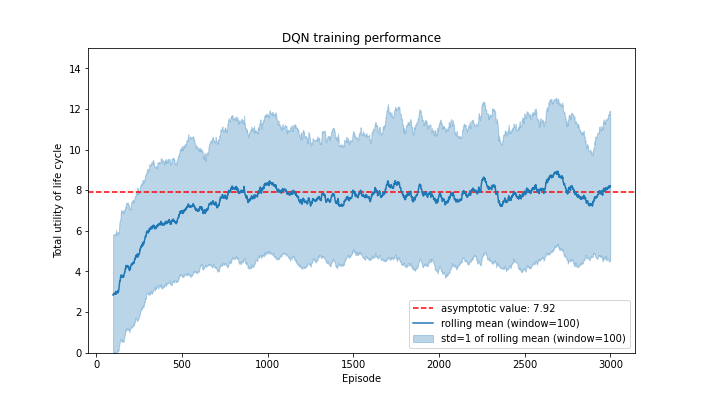
\includegraphics[width=1\linewidth]{figures/dqn_training_performance_simple_model.png}
  \caption{DQN Training Performance}
  \label{fig:dqn_training_performance_simple}
\end{subfigure}%
\begin{subfigure}{.5\textwidth}
  \centering
  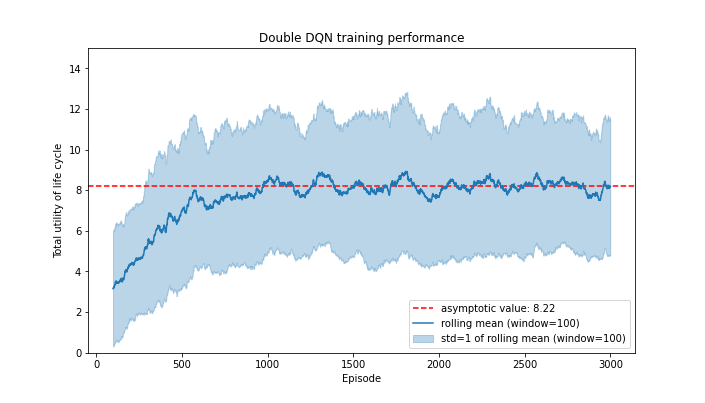
\includegraphics[width=1\linewidth]{figures/ddqn_training_performance_simple_model.png}
  \caption{Double DQN Training Performance}
  \label{fig:ddqn_training_performance_simple}
\end{subfigure}
    \caption{Comparing training perfance of Deep Q-Learning and Double Deep Q-Learning}
    \label{fig:training_performance_simple_model}
\end{figure}

Figure \ref{fig:dqn_solution_beta2} and \ref{fig:dqn_solution_beta4} compares the performance of the algorithm to two different benchmarks. One benchmark is the environment with a $\beta_L = 2$ another $\beta_L=4$. These differences in preferences will yield different optimal policies conditional on the $\beta_L$. I compare the policy chosen by the agent with different deterministic policies. Figure \ref{fig:dqn_solution_beta2} (left plot) shows either using $0, 37, 45$ hours pr. week as comparisons and an agent picking randomly. All agents have been simulated for 300 episodes, yielding the plots being averages, and the standard deviations are calculated on a pr. age basis for each agent. It should also be noted that $\epsilon$ (the exploration ratio of the agent) is set to 0, such that the agent now only greedily navigates the environment. Comparing this to the VFI agent I find  it reasonable to assume that the DQN agent has learned to navigate the environment. A small dip from around age 55 can be observed, but I believe this does not make the feat any less impressive, and furthermore I believe that the solution fairly accurately approximates the correct optimal policy. Looking to the the right hands side plot, the variance of the utility (1 standard deviation). Again the best benchmark for $\beta_L = 2$ an agent that works 45 hours a week, seem have a overlap even in the last periods, where they diverge a little, allowing me to conclude, that this differences in performance is very small. Figure \ref{fig:dqn_solution_beta4} shows the same plot just for $\beta_L = 4$. Again the DQN agent fairly accurately approximates the optimal policy, with even less variance than observed in with $\beta_L = 2$. One thing to note is, that a small hump can be observed for the DQN agent at around age 28, where it has found a way to beat the deterministic policy. Again this might just be variance of the simulations. 


\begin{figure}[ht]
\begin{subfigure}{.5\textwidth}
  \centering
  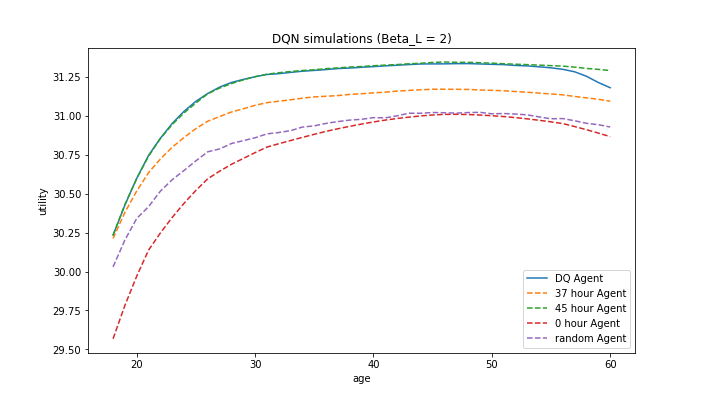
\includegraphics[width=1\linewidth]{figures/dqn_model1_beta_2_solution_benchmark_paths.png}
  \caption{Simulated Paths}
  \label{fig:dqn_solution_beta2_path}
\end{subfigure}%
\begin{subfigure}{.5\textwidth}
  \centering
  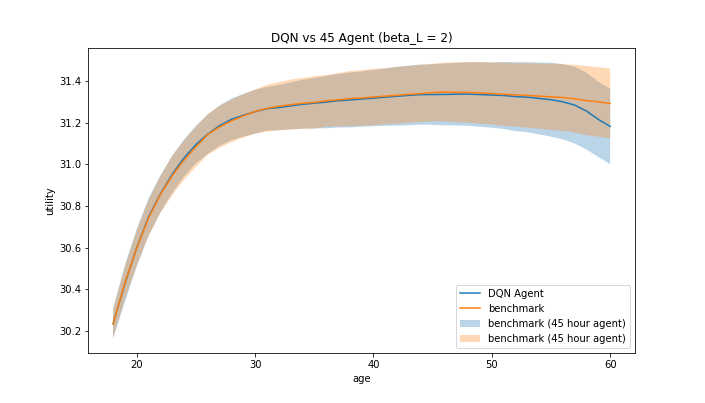
\includegraphics[width=1\linewidth]{figures/dqn_model1_beta_2_solution_benchmark_variance.png}
  \caption{Variance of Paths}
  \label{fig:dqn_solution_beta2_var}
\end{subfigure}
    \caption{Deep Q-Learning solution vs. benchmark $(\beta_L = 2)$}
    \label{fig:dqn_solution_beta2}
\end{figure}

\begin{figure}[ht]
\begin{subfigure}{.5\textwidth}
  \centering
  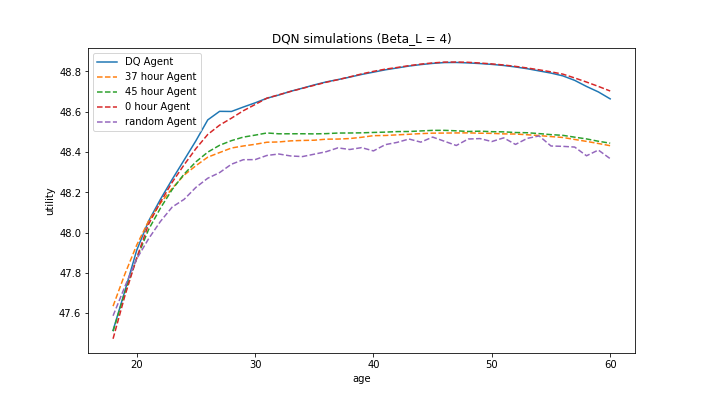
\includegraphics[width=1\linewidth]{figures/dqn_model1_beta_4_solution_benchmark_paths.png}
  \caption{Simulated Paths}
  \label{fig:dqn_solution_beta4_path}
\end{subfigure}%
\begin{subfigure}{.5\textwidth}
  \centering
  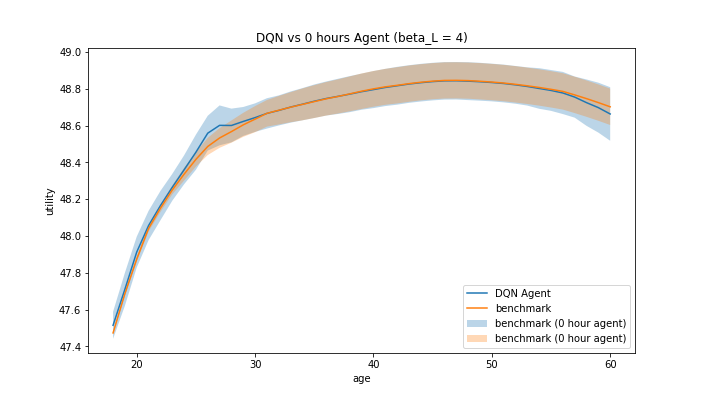
\includegraphics[width=1\linewidth]{figures/dqn_model1_beta_4_solution_benchmark_variance.png}
  \caption{Variance of Paths}
  \label{fig:dqn_solution_beta4_var}
\end{subfigure}
    \caption{Deep Q-Learning solution vs. benchmark $(\beta_L = 4)$}
    \label{fig:dqn_solution_beta4}
\end{figure}


\subsection{Double Deep Q-learning}

Deep Q-learning is good starting point for a learning algorithm using non-linear function approximation, however certain properties of the algorithm is problematic. \parencite{van_hasselt_deep_2015} argues this is mainly due to the fact that Deep Q-learning can tend to be overoptimistic in a problematic way. In general there exists two ways in which overoptimism can be good or at least not detrimental to performance. 1) If the algorithm uniformly overestimates the Q-function for all actions, then this is not associated with any problems, since taking the max of the Q-function w.r.t. to the action, will lead to the same result had the estimations been correct. In other words, performance would not change, however introspection of the algorithm might be harder. 2) It can be a good thing for an algorithm to be optimistic when faced with uncertainty. If an action would lead to observing an unexplored part of the state space, it might be a good thing to be optimistic with regards to exploration, allowing for possible new policies with higher yielding returns over the episode. Deep Q-learning do not conform to any of these properties, instead it usually overestimates the value of the action it has taken due to the max operator in the value estimation: $R_{t+1} + \gamma \underset{A_{t+1}}{\argmax} Q(S_{t+1}, A_{t+1})$. A simple extension presented by \textcite{van_hasselt_deep_2015} is to decouple the prediction with the evaluation. This can be done by having two different sets of weights, where one $\theta$ is used for the policy (policy weights) and one $\tilde{\theta}$ is used for the evaluation (target weights). This can be presented the following way. The Q-network target:

\begin{equation}\label{eq:dqn_target}
    Y_t^{Q} = R_{t+1} + \gamma Q(S_{t+1}, \underset{a}{\argmax} (S_{t+1}, a ; \theta) ; \theta)
\end{equation}

and the Double DQN target is calculated:

\begin{equation}\label{eq:ddqn_target}
    Y_t^{DoubleQ} = R_{t+1} + \gamma Q(S_{t+1}, \underset{a}{\argmax}Q(S_{t+1}, a; \theta); \tilde{\theta}) 
\end{equation}

This alleviates the problem of overestimating the values returned by the algorithm for the following reason. Consider \eqref{eq:dqn_target}. When calculating the value of the state action pair, one uses the same function to choose the action, prompting  a real risk of overestimation of the state action pair of the chosen action. The equation below \eqref{eq:ddqn_target} instead estimates the value of the position by using a different set of parameters, $\tilde{\theta}$. Following the implementation of \textcite{van_hasselt_deep_2015} instead of training 2 separate networks the target weights are inherited from the evaluation weights. This is to reduce time of training the algorithm, even though the policy and target network can not be considered perfectly decoupled then. The implication of this design choice is $\tilde{\theta} = \theta^{previous}$, such that, the target estimation is made by the old weights, while the value of greedy policy uses the new weights:

\begin{equation}\label{eq:ddqn_target_final}
    Y_t^{DoubleQ} = R_{t+1} + \gamma Q(S_{t+1}, \underset{a}{\argmax}Q(S_{t+1}, a; \theta_t); \theta_t^{previous}) 
\end{equation}

The full algorithm, which to large extend mirrors the algorithm for Deep Q-learning is presented in algorithm \ref{alg:ddqlearning}:

\begin{algorithm}[H]
\SetAlgoLined
 Initialize replay memory $\mathcal{D}$ with capacity $N$\;
 Initialize action-value function $Q$ with random weights: $\theta, \tilde{\theta}$\;
 Initialize memory counter $j \leftarrow 1$\;
 Initialize $k$ when to replace target weights $\tilde{\theta}$\;
 \ForEach {episode $\in \{1, 2, \cdots M \}$}{
  Initialize sequence with an initial state $s_1$. This is drawn randomly.\;
    \For{$t \in \{1, 2, \cdots, T$ \}}{
    With probability $\epsilon$ select a random action $a_t$\;
    Otherwise select $A_t = \underset{a}{\argmax}Q^*(S_t, A_t ; \theta)$\;
    Execute action $A_t$ in environment and observe reward $R_t$ and the new state $S_{t+1}$\;
    Store transition $(S_t, A_t, R_{t+1}, S_{t+1})$ in $\mathcal{D}$\;
    Sample random mini-batch of transitions $(S_t, A_t, A_{t+1}, S_{t+1})$ from $\mathcal{D}$\;
    Set $
      Y_j = \begin{cases}
        R_j & \text{if terminal states} \\
        R_j + \gamma Q(S_{t+1}, \underset{a}{\argmax} Q(S_t, a; \theta_t); \tilde{\theta_t}) & \text{if non-terminal states}
      \end{cases}
    $ \;
    Perform gradient descent step on $(Y_j - Q(S_t, A_t ; \theta))^2$ w.r.t $\theta$ \;
    If $j$ is divisible by $k$ replace target weights $\tilde{\theta} \leftarrow \theta$\;
    Increment $j$ \;
  }
}
\caption{Double Deep Q-learning}
\label{alg:ddqlearning}
\end{algorithm}

Just as with the Deep Q-learning implementation i let the Q-function map from: $\statespace \mapsto \R^{\mid \actionspace \mid}$, to reduce the number of computations, when taking the max over the Q-function. 


For the Double DQN agent I in general use the same hyper parameters used for the DQN agent: The network architecture is again an input layer of the size of the state space, followed by two fully connected layers with Rectified Linear units as activation functions ending with an output layer with linear activation of same size as the action space. Again i let the learning rate be $\alpha = 0.0005$ and the $\epsilon_i = \max (\epsilon_{i-1} \cdot 0.9999, 0.01)$, such that exploration is performed through out the training period. Again the replay buffer has a capacity of a million rows and i use mini batches of size 64 to perform stochastic gradient descent on the weight of the neural network approximating the Q-function. I transform the states such that they are mean zero and a standard deviation of 1. The same is true for the rewards conditional on the $\beta_L$ value. The $\beta_L$ value is just as with $DQN$ and value function iteration added to the state space, allowing for a single solution of the model. I uniformly draw $\beta_L$ from the interval $[0.2, 6]$ and sets this to be part of the environment in the beginning of each episode. I use the Adam optimizer when updating the weights using gradient descent. I let the target network inherit the old weights every 100'th iteration of the algorithm. The algorithm is trained for 3000 episodes. Figure \ref{fig:training_performance_simple_model} (right plot) shows the performance. Very similar to the DQN I find that the performance stabilized at around 1000 episodes, and reaches an asymptotic performance of $8.22$, which is slightly higher compared to the DQN agent which had an asymptotic value of $7.92$.

\begin{figure}[ht]
\begin{subfigure}{.5\textwidth}
  \centering
  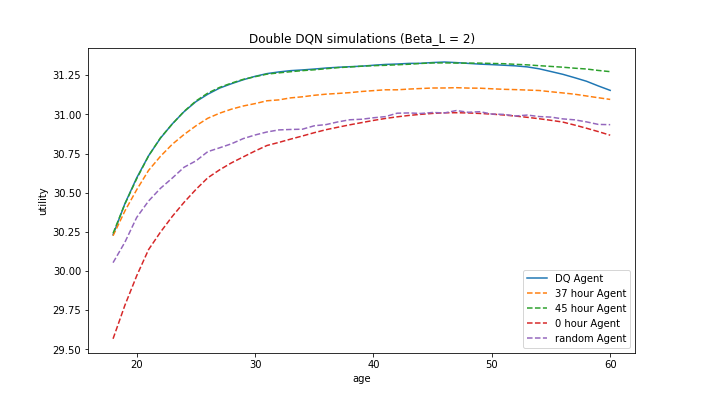
\includegraphics[width=1\linewidth]{figures/ddqn_model1_beta_2_solution_benchmark_paths.png}
  \caption{Simulated Paths}
  \label{fig:ddqn_solution_beta2_path}
\end{subfigure}%
\begin{subfigure}{.5\textwidth}
  \centering
  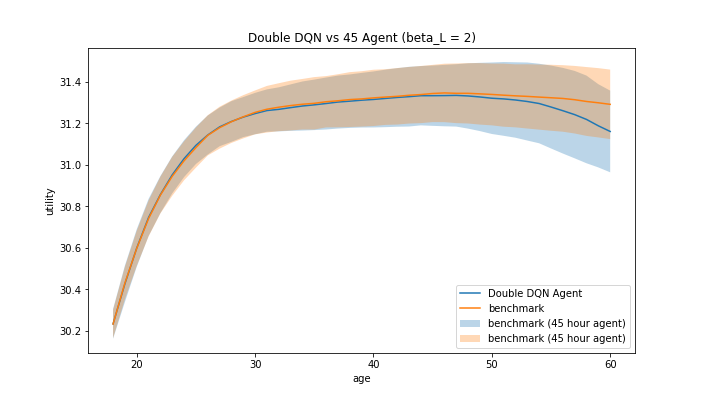
\includegraphics[width=1\linewidth]{figures/ddqn_model1_beta_2_solution_benchmark_variance.png}
  \caption{Variance of Paths}
  \label{fig:ddqn_solution_beta2_var}
\end{subfigure}
    \caption{Double Deep Q-Learning solution vs. benchmark $(\beta_L = 2)$}
    \label{fig:ddqn_solution_beta2}
\end{figure}

\begin{figure}[ht]
\begin{subfigure}{.5\textwidth}
  \centering
  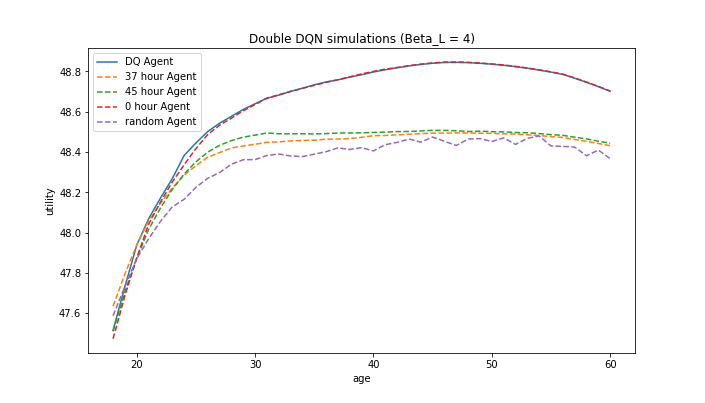
\includegraphics[width=1\linewidth]{figures/ddqn_model1_beta_4_solution_benchmark_paths.png}
  \caption{Simulated Paths}
  \label{fig:ddqn_solution_beta4_path}
\end{subfigure}%
\begin{subfigure}{.5\textwidth}
  \centering
  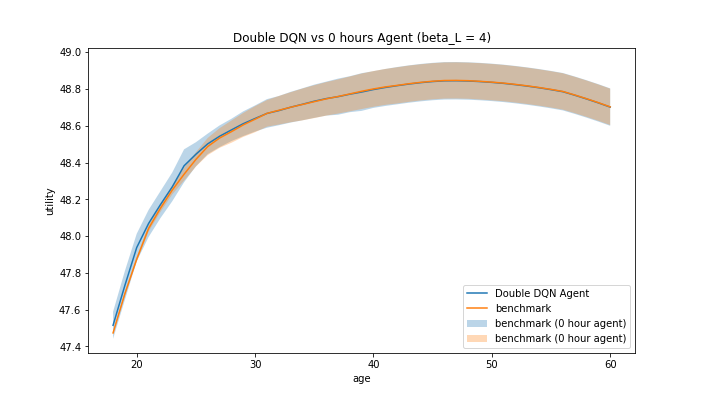
\includegraphics[width=1\linewidth]{figures/ddqn_model1_beta_4_solution_benchmark_variance.png}
  \caption{Variance of Paths}
  \label{fig:ddqn_solution_beta4_var}
\end{subfigure}
    \caption{Double Deep Q-Learning solution vs. benchmark $(\beta_L = 4)$}
    \label{fig:ddqn_solution_beta4}
\end{figure}

Figure \ref{fig:ddqn_solution_beta2} and \ref{fig:ddqn_solution_beta4} shows the performance of the Double DQN agent comparing it to two different preferences of leisure: $\beta_L = 2$ and $\beta_L = 4$. Four agents is used for comparison: An agent that chooses actions randomly, and three agents that in an deterministic fashion works $0, 37$ or $45$ hours a week. The results of the Double DQN agent is comparable to those found within the other agents (VFI and DQN). Figure \ref{fig:ddqn_solution_beta2} shows the performance where the preference for leisure $\beta_L = 2$. Again the best deterministic policy is the 45 hour agent, which is very close to what the DQ agent chooses, except for the last 5 years of the agent's life cycle where the utility is slightly lower. Comparing the variance of the utility on right hand side plot of figure \ref{fig:ddqn_solution_beta2}, there is overlap of the simulations of the Double DQN agent and the 45 hours a week agent. Figure \ref{fig:ddqn_solution_beta4} compares the Double DQN agent to the agents when the preference for leisure $\beta_L = 4$. Here again the optimal policy pretty closely mirrors the best deterministic agent, the one which does not work, with a clear overlap presented in figure on right hand side.


\section{Estimation}

Only a single parameter of the model needs to be estimated: $\beta_L$. For this estimation, method of simulated moments is employed.  \textcite{eisenhauer_estimation_2015} suggests a diagonal matrix as a standard choice of weight matrix when using methods of moments, allowing for writing the estimation as the sum of squared errors between the simulated and empirical moments. Phrased differently: the objective function minimizes the mean squared error (MSE) between the empirical moments and the simulated. Since I use aggregate data from Statistics Denmark, I have not access to the standard errors of the estimates of the empirical moments usually used for the weight of the individual moments. Instead I weigh each moment equally. Since this application relies on grid search over the single parameter $\beta_L$, I choose the $\beta_L$ corresponding to the lowest loss of the objective function. 

Usually when estimating a structural model using simulated methods of moments one would not supply the parameters as part of the state space. The reason for this is, that as the size of the state space expands, it gets exponentially more expensive to solve the model. The algorithm would go: For a given set of parameters needed to be estimated, supply a random initialization. Solve the model for given parameters. Use the solved model to calculate the moments. Use numerical optimization to minimize given optimization problem. However in this application I have chosen to make the parameter part of the state space, since this paper tries to establish that high dimensional dynamic models can be solved using Deep Reinforcement Learning, and therefore not being a limited by the size of the state space.

This paper has implemented the following strategy for estimating the model: I create a grid of 50 points with $\beta_L$ values in the range $[0.2, 8]$ evenly spaced. I simulate $N=300$ agents for a given value of $\beta_L$ in the grid. Using the 300 agents the mean number of supplied hours pr. agent can be calculated. Here it is important to note, that if an agent works 0 hours, the agent is assumed to be out of the workforce and not appear in the statistics, therefore the objective function is:

\begin{equation}
    \text{Objective} = \sum_{q=Q_{\min}}^{Q_{\max}} \lsp \mu_{q} -\frac{1}{\sum_{i=1}^{N} \mathbf{1}\{H_{i,q} > 0\}}\sum_{i=1}^N (H_{i,q})\rsp^2
\end{equation}

Where $q$ denotes the age of an individual agent and $i$ denotes an individual. $\mu_q$ is the empirical average of supplied ours of women of a age 	$q$. Again I use \textbf{LIGEF15} supplied by Statistics Denmark to get the average number of supplied of hours. I use the same seed for the simulation, every time the $N$ agents is simulated with a new $\beta_L$ value. The estimation is performed for each of the solution methods in this paper: Value function Iteration, Deep Q-Learning and Double Deep Q-Learning. 

The estimation yields the following optimal values using VFI: $\beta_L=3.43$, Optimal Values using DQN $\beta_L=3.59$ and optimal value of Double DQN $\beta_L=3.59$. $3.43$ and $3.59$ are neighbouring grid points. I believe it is safe to conclude that these methods yields if not identical, then almost identical results, and I am willing to conclude that Deep Q-Learning and Double Deep Q-Learning are excellent methods for solving dynamic models - at least in this setting!

\begin{table}[ht]
    \centering
    \begin{tabular}{lrrr}
\toprule
{} &  VFI &  DQN & Double DQN \\
\midrule
$\hat{\beta_L}$ & 3.43 & 3.59 & 3.59 \\
\bottomrule
\end{tabular}
    \caption{Estimation of $\beta_L$}
    \label{tab:beta_L_Estimation}
\end{table}

Looking to figure \ref{fig:beta_L_estimation} it can be seen that the estimations follow the same trajectory. The plot shows the log(MSE) for $\beta_L$ values in the range $[0.2, 8]$. Starting with low $\beta_L$ having medium high MSE, falling slightly at around $\beta_L = 3$ reaching a minimum at about $\beta_L = 3.5$, and after that a sharp raise in MSE is observed. 

\begin{figure}[ht]
\begin{subfigure}{.5\textwidth}
  \centering
  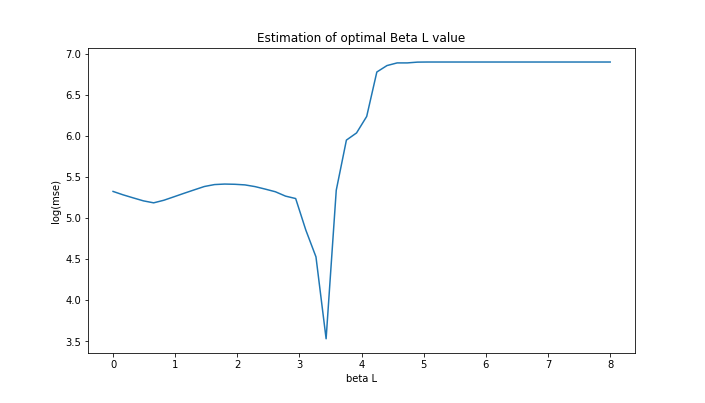
\includegraphics[width=1\linewidth]{figures/dqi_model1_estimation_Beta_L.png}
  \caption{Value Function Iteration Estimation of $\beta_L$}
  \label{fig:dqi_estimation_beta_L}
\end{subfigure}%
\begin{subfigure}{.5\textwidth}
  \centering
  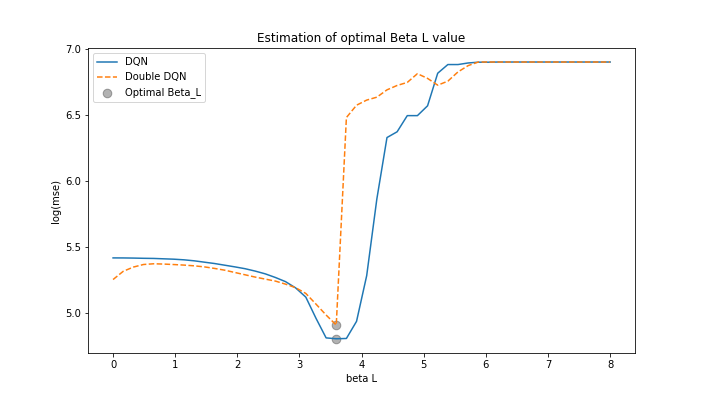
\includegraphics[width=1\linewidth]{figures/dqn_ddqn_model1_estimation_Beta_L.png}
  \caption{DQN and Double DQN estimation of $\beta_L$}
  \label{fig:dqn_ddqn_estimation_beta_L}
\end{subfigure}
    \caption{Estimation of $\beta_L$}
    \label{fig:beta_L_estimation}
\end{figure}



\section{Results}

I arbitrarily choose value function iteration when investigating the results of the model, since all the solution methods yielded identical results. 5000 agents is simulated using the optimal $\beta_L = 3.43$. Relevant summary statistics can be calculated over the 5000 simulations. The statistics can be used to infer whether or not the model fit the data and compare to what is expected from the real world. Looking to figure \ref{fig:dqi_model1_average_path_sim_vs_empirical} the empirical number of hours supplied by women \textbf{LIGEF15} is compared to the simulated. Again only women actually in the labour force  ($H>0$) is considered. The fit of the data does seem reasonable. In general the simulated data set slightly overestimates the number of supplied hours. Especially around age 30 does the simulated number of supplied hours seem to be higher than the empirical. The simulated data show heterogeneity over the life cycle, where especially the later stages of the life cycle show higher variance. This could very well stem from the idiosyncratic wage path increasing over time. Considering the estimation method relied on the number of supplied hours, it is not surprising that this is where the model performs the best. 


\begin{figure}
    \centering
    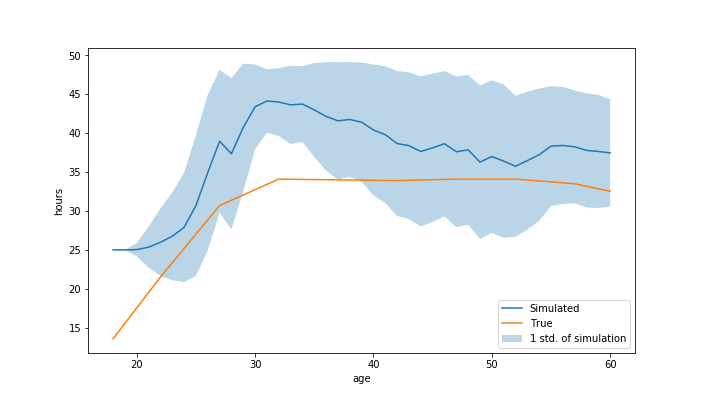
\includegraphics[scale=0.4]{figures/dqi_model1_estimation_labour_supply.png}
    \caption{Average Number of Supplied Working Hours - Empirical Vs. Simulated}
    \label{fig:dqi_model1_average_path_sim_vs_empirical}
\end{figure}

Figure \ref{fig:dqi_model1_fraction_in_workforce} shows the participation rate of women in the workforce in the simulated data set. From here it is very clear, that the model underestimates the number of women working! From age 25, 80 \% of the women is out of the workforce, followed by a slow decline in participation going forward to retirement. This does obviously not correspond to what can be observed in the real world. Even though it is not possible to get access to the exact number of women out of the labour force conditional on age, it can be approximated. Using \textbf{FOLK1B} supplied by Statistics Denmark the number of women in the age (15 to 60) can be found. Using that data the number of relevant women (considering the age) is around 1.664 million people. The number of women not working for relevant reasons can be summarized to: women not working due to: \textit{working in the home}, \textit{Studying}, \textit{Other people outside the labour force}. These add up to: $15 + 161 + 66 = 242$ thousand people or $0.242$ million people. The number of women in the relevant age group outside the labour force can be approximated to the number given in equation \ref{eq:women_outside_the_labour_force}

\begin{equation}
    \label{eq:women_outside_the_labour_force}
    \textbf{Women outside the labour force} = \frac{0.242}{1.664} = 0.145 = 14.5 \% \approx 15 \%
\end{equation}

The estimation of $\beta_L$ did not take this measure into account, which might be a way to improve the results.

\begin{figure}
    \centering
    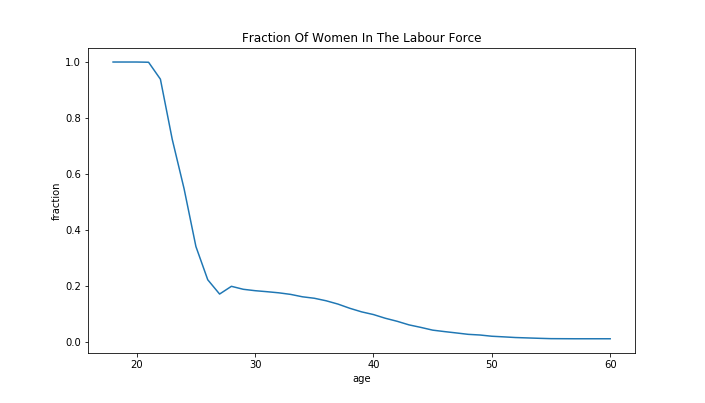
\includegraphics[scale=0.4]{figures/dqi_model1_women_in_labour_force_fraction.png}
    \caption{Fraction of Women in The Labour Force}
    \label{fig:dqi_model1_fraction_in_workforce}
\end{figure}

Both figure \ref{fig:dqi_model1_birth_onset} and figure \ref{fig:dqi_model1_child_vs_no_child_30} is inspired by the article of \textcite{kleven_children_2019}. In the article the authors show how participation of a woman is affected when she gives birth to a child. In the paper they find that women,  when giving birth to a child on average use 20 \% time less on work, compared to the husband, immediately after the birth of the child. The number of supplied hours slowly return to steady state with a long run penalty of around 6 \%. This is not the case for the simulated household. Getting a child, do seem to decrease the number of hours supplied however, the difference is indistinguishable from the mothers not getting children. This is clear in figure \ref{fig:dqi_model1_child_vs_no_child_30}, where first time mothers of age 30 is compared to women that have no children. The paths are indistinguishable, where the paper by \textcite{kleven_children_2019} would suggest a decrease of about 20 percent immediately after the birth (at age 31). These figures do not sort out women outside the labour force. I conclude the model is insufficient to capture the real world, and I move on to extend this original model.


\begin{figure}[ht]
\begin{subfigure}{.5\textwidth}
    \centering
    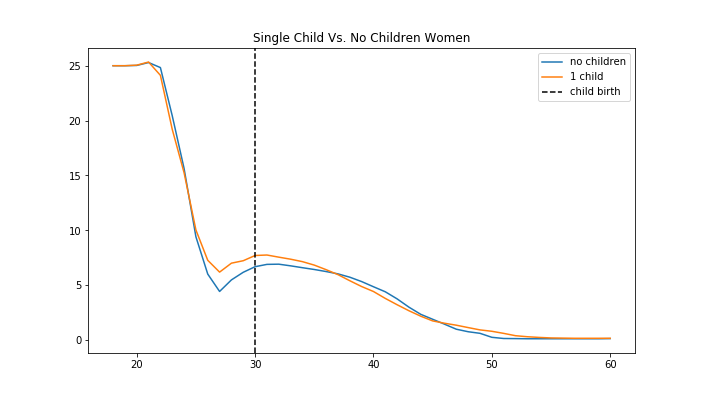
\includegraphics[width=1\linewidth]{figures/dqi_single_child_vs_no_child_model1.png}
    \caption{First time mothers vs. Women with no children}
    \label{fig:dqi_model1_child_vs_no_child_30}
\end{subfigure}%
\begin{subfigure}{.5\textwidth}
    \centering
    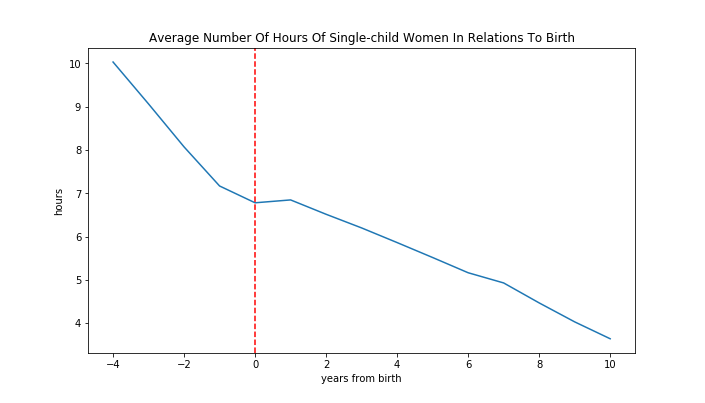
\includegraphics[width=1\linewidth]{figures/women_supplied_hours_dqi_model1_birth_onset.png}
    \caption{hours compared to birth onset.}
    \label{fig:dqi_model1_birth_onset}
\end{subfigure}
    \caption{Impact of Children}
    \label{fig:model_impact_children}
\end{figure}



\section{Model (Extended)}

This will be where the extended model will be.

\section{Solving and Estimating the extended Model}

\subsection{Solution}

For this extended model I only use the Double Deep Q-Network agent, since it was shown with the simpler model, this model has comparable performance to the VFI implementation and Deep Q-network. The model is solved by running 3000 episodes. As was true for the simple model, the deep learning algorithm performs best if states are scaled mean 0 and a standard deviation of 1. In practice this is done by applying a transformer in my agent that can do a scaling of the states. Furthermore the scaling is capable of doing an inverse transformation. The rewards are also scaled, this slightly improves performance, but the primary reason is, that it helps track the learning. I scale the rewards to have a variance of about 1, and let them have the same mean conditional of the $\beta_L$  value! I train the algorithm for 3000 episodes, have the hyper parameters of the algorithm being: $\gamma=0.99$ representing the impatience of the agent. The agent is initialized with $\epsilon=1.0$ which decays by $0.9999$ for each step the agent performs. The learning rate is $\alpha=0.0005$. The size of the memory buffer is one million rows, and I train with a batch size=64. I let the minimum exploration rate in training be $0.01$. I let the architecture of the network be identical to the simpler model: An Input layer of same size as the state space, 2 fully connected layers of size 256 with rectified linear units as activation functions, and an linear output layer of the same size as the action space. At the beginning of each episode a random $\beta_L \sim Uniform(0, 60)$, allowing the agent to step through an episode until terminal with given $\beta_L$. Finally the target network inherits the policy weights every $100$'th step. A score for every 50'th episode is run, taking the average of the previous 50 episodes. If the current iteration of the model beats the high score, the weights of the neural network is saved. The estimation and simulation is performed with the weights that yield the highest score for 50 consecutive episodes. 

\begin{figure}[ht]
    \centering
    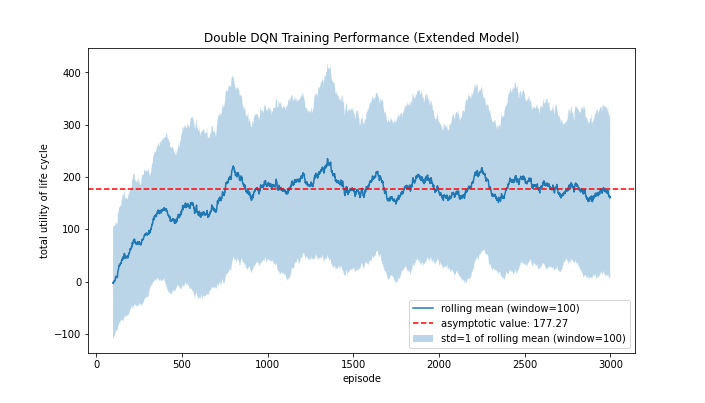
\includegraphics[scale=0.4]{figures/ddqn_extended_model_training_performance.png}
    \caption{Estimation of $\beta_L$ for extended model}
    \label{fig:training_extended}
\end{figure}

Looking to figure \ref{fig:training_extended} the agent clearly learns to navigate in the environment. After about 1000 episodes the agent seems to have learned to navigate the environment! The maximum score appears at around episode 1400, which is the weights used for estimation and simulations. The asymptotic training performance is about 177 compared to an initial score of approximately zero.

\subsection{Estimation}

As was the case with the simpler model, only a single parameter $\beta_L$ needs to be estimated. Again, just as was the case before with the simpler model, I have extended the state space with $\beta_L$. I use a grid search in the range $\beta_L \in [0, 60]$, simulating $N=800$ observations, calculating the objective function. I use the same seed in each iteration of the optimization process. To address the short comings of the simple model i expand the objective function of the optimization problem. In the initial model too many women choose not to be part of the labour force yielding unrealistic results. Therefore the objective function now extends to two broad goals: Have the right number of women be out of the labour force (around 15 \%) and fit the curve of number of working hours for women. The first objective, \textit{objective 1}, is formulated as: 

\begin{equation}
    \text{objective 1} = \lsp\frac{\sum_{i=1}^{N} \sum_{q=Q_{\min}}^{Q_{\max}} \mathbf{1}\{H_{i,q} = 0\}}{ N \cdot (Q_{\max} - Q_{\min} )} - 15\% \rsp^2
\end{equation}

The second objective is formulated the same way as it was when first estimating the simple model, which correspond the conditional expectation of supplied number of working hours conditional on the age and of being in the labour force $ \E[H \mid Q=q, H>0]$. The desired outcome is for this to be true for all ages from 18 to 60, $\mu_q$ is the empirical moment found using the data \textbf{LIGEF15}:

\begin{equation}
    \text{Objective 2} = \sum_{q=Q_{\min}}^{Q_{\min}} \lsp \mu_q  - \frac{1}{\sum_{i=1}^{N} \mathbf{1}\{H_{i,q} > 0\}}\sum_{i=1}^N (H_{i,q})\rsp^2
\end{equation}

Now this description of the objectives can be translated into a more formal formulation. The number of moments are $\text{\# moments}  = 1 + (Q_{\max} - Q_{\min}) = 1 + 60 - 18 = 43$. Now the weighting of these moments would usually be done by some weight matrix $W$ in a formula looking like: $[\hat{m} - \tilde{m}]^{\top} W^{-1} [\hat{m} - \tilde{m}]$, where $\tilde{m}$ is a vector of empirical moments and $\hat{m}$ is a vector of simulated moments allowing for the methods of moments estimation. The choosing of the weight matrix is application specific. \textcite{eisenhauer_estimation_2015} suggests the choice in that setting should be the inverse variance of the empirical moments $\tilde{m}_j$, on the diagonal of the weight matrix (zeros else), letting the $j$'th moment correspond to the $j$'th weight. This is however not possible in this application, due to the fact, that I only have access to aggregated data from statistics Denmark. Instead i manually chooses scales such that \textit{objective 1} is equally weighted to \textit{objective 2}. This first and foremost requires a scaling of the moments. And second of all this requires a re-weighing since there are 42 moments composing \textit{objective 2} and only a single moment composing \textit{objective 1}. Since the distance between the empirical and the simulated moment is squared, the scaling must be performed before the squaring. Finally, since the weight matrix is chosen as it is, a transformation can be performed such that instead of a matrix product it can be considered a sum: $\sum_{j = 1}
^{43} ( \hat{m}_j - \tilde{m}_j )^2$, becoming a mean squared error optimization problem. It is implied that $N$ agents is simulated conditional on a value of $\beta_L$. The objective function does in other words look as:

\begin{multline}
   \text{Objective}(\beta_L) =  \lsp 37 \cdot \lp\frac{\sum_{i=1}^{N} \sum_{q=Q_{\min}}^{Q_{\max}} \mathbf{1}\{H_{i,q} = 0\}}{ N \cdot (Q_{\max} - Q_{\min} )} - 15\% \rp \rsp^2 \\ + \frac{1}{Q_{\max} - Q_{\min}}\sum_{q=Q_{\min}}^{Q_{\max}} \lsp \mu_q - \frac{1}{\sum_{i=1}^{N} \mathbf{1}\{H_{i,q} > 0\}}\sum_{i=1}^N (H_{i,q})\rsp^2
\end{multline}

\begin{figure}[ht]
    \centering
    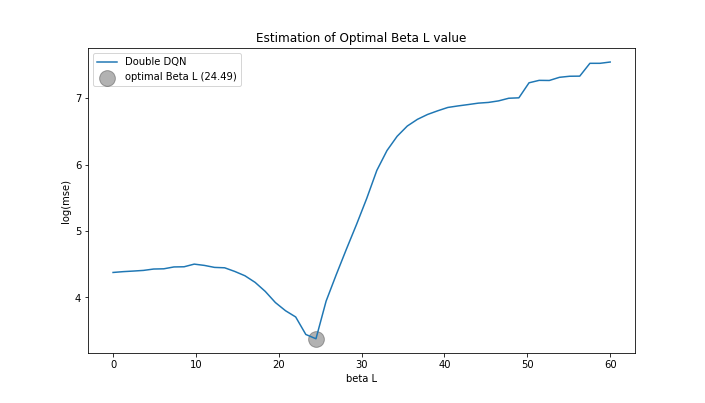
\includegraphics[scale=0.4]{figures/ddqn_extended_model_estimation_beta_L.png}
    \caption{Estimation of $\beta_L$ for extended model}
    \label{fig:estimation_extended}
\end{figure}

The estimated value of $\beta_L = 24.49$. Figure \ref{fig:estimation_extended} shows the grid search, and finds that optimization problem, contains a minimum at $\beta_L = 24.49$, suggesting that the range of the grid is adequate for the estimation problem. I take the $\log (\cdot)$ of the mean squared error to better represent it in figure \ref{fig:estimation_extended}, allowing for not showing the less extreme tails.

\section{Results of the Extended Model}

I simulate 200.000 households using the optimal $\beta_L = 24.49$. Using the simulations a counter factual analysis of households that do get children, compared to households that do not can be made. Figure \ref{fig:ext_model_working_hours} shows the average number of working hours of the simulations compared to the empirical number of hours worked by women. This extended model fits the data considerably better than the simple model, as shown in figure \ref{fig:dqi_model1_average_path_sim_vs_empirical}. Again the models also differ in the action space, where this extended model do not allow for working more than 37 hours a week. The average number of hours worked is conditional on the supplied number of hours working must be above 0. The figure also shows the average number of hours supplied by women when they get children at their specific age. This is true for age 25, 30 and age 35. These households get one child and only one child, where I do not condition on $H>0$. Looking to these households steep dips in the supplied number of hours are present, at about 5 hours for each of the three age groups. The cohorts of households that get a child at age 30 and 35 year dip to a permanently lower number of supplied hours, whereas the cohort that get a child at age 25, get an initial dip, but readjust after a certain period. For all three cohorts the initial dip, the households experience, has a magnitude of about 5 hours.

\begin{figure}
    \centering
    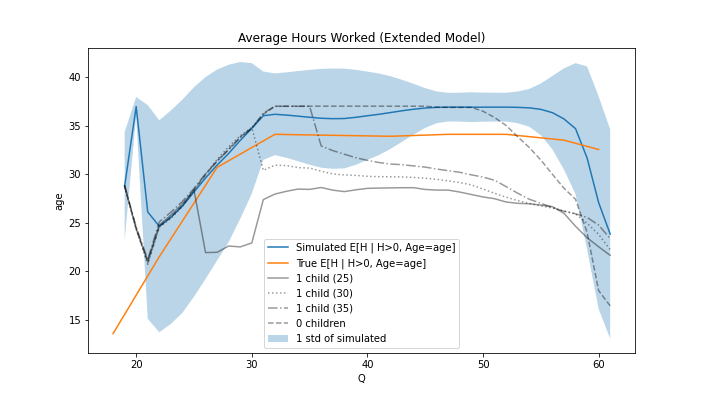
\includegraphics[scale=0.4]{figures/extended_model_average_hours.png}
    \caption{Extended Model Working Hours - Empirical Vs. Simulated}
    \label{fig:ext_model_working_hours}
\end{figure}

Figure \ref{fig:ext_model_particpation_rates} shows the participation rate over the life cycle. The average participation of all simulations is $81.7 \%$ letting the overall number of women out of the workforce be equal to $18.3 \%$. Comparing to the number used for the estimation of $\beta_L$, which was $15 \%$, the results must be considered a good fit. I have not found good data from Statistics Denmark showing women's average participation rate over the life cycle, implying it is hard to make inference over the participation rate over the life cycle, however, a couple of things can be noted. First and foremost the simulations show a downward sloping trend of participation rates over the life cycle. \textcite{grimm_labour_2001} have investigated female labour participation rate in France over the life cycle. The data  they present suggests this picture is not entirely unrealistic. One thing should be noted about the comparison. Their sample ends in 1998, and looking to that data, the downward sloping trend do seem to be less pronounced comparing to earlier generations. I have shown four different cohorts in the same figure. As before I have focused on families getting 0 children, a cohort of households getting a child at age 25, a cohort of households getting a child at age 30, and lastly a cohort of households getting their first and only child at age 35. The picture is clear, when the child is born, it has a very strong effect on participation rate. Households getting a child at age 25, do seem to have a penalty of 30 percent reduction in participation rate for the next five years. Families getting their child at age 30 experience a reduction in participation rate slightly below 20 percent, and at last the cohort of households getting a child at age 35 experience a reduction in participation rate at around 10 percent.

\begin{figure}
    \centering
    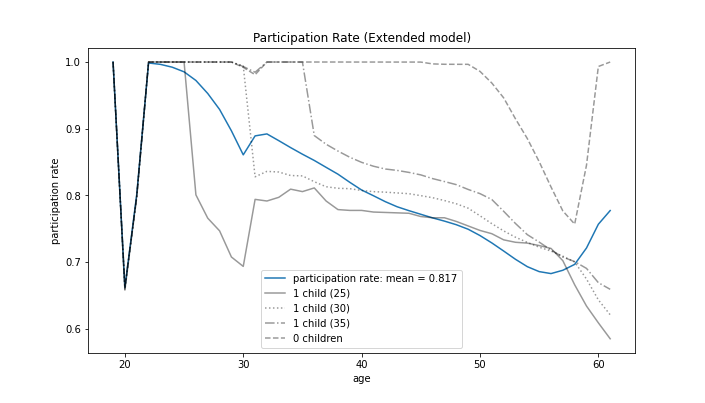
\includegraphics[scale=0.4]{figures/extended_model_participation_rates.png}
    \caption{Participation rates}
    \label{fig:ext_model_particpation_rates}
\end{figure}

Figure \ref{fig:ext_model_impact_earnings_hours} and \ref{fig:ext_model_impact_participation_wage} displays event graphs of households getting a (single) child at different ages. These are compared against the women of households that do not get children. These event graphs compares to the event graphs by \textcite{kleven_children_2019}, however there are a couple of differences. \textcite{kleven_children_2019} considers the husband of the household as benchmark whereas I consider women of households with no children the benchmark. The husband of the household, in this model, is considered to follow a deterministic path, and household heterogeneity only comes from the different choices of the woman of the household, letting this be a more natural comparison for this model. Comparing the results, even though the benchmarks do diverge, does lead to surprisingly similar conclusions. First notice that the earnings do seem to have the largest reduction for households that get children at an early age. The same goes for hours worked, participation rates and wage rates. Secondly the long run penalties do converge to approximately the same levels. Table \ref{tab:extended_results} lists the different long run penalties compared to \textcite{kleven_children_2019}. Comparing the long run penalties, this analysis find 5 percentage points lower long run penalties for earnings, 10 percentage points higher penalty for hours works, 8 percentage points higher penalties for participation rates and 14 percentage points lower penalty for wage rates in this model than the results found by \textcite{kleven_children_2019}.

\begin{figure}[ht]
\begin{subfigure}{.5\textwidth}
  \centering
  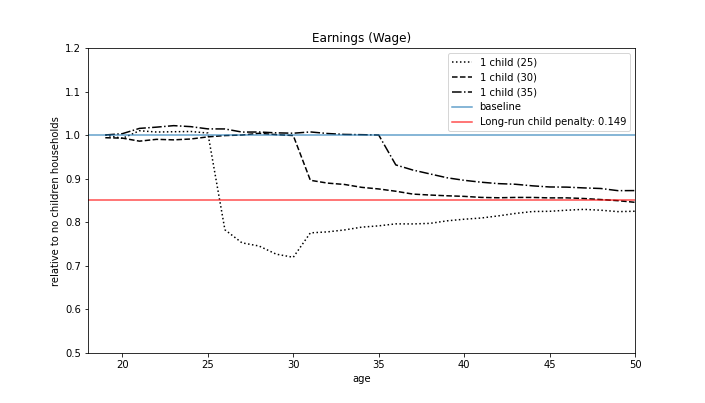
\includegraphics[width=1\linewidth]{figures/extended_model_event_earnings.png}
  \caption{Earnings}
  \label{fig:ext_model_event_earnings}
\end{subfigure}%
\begin{subfigure}{.5\textwidth}
  \centering
  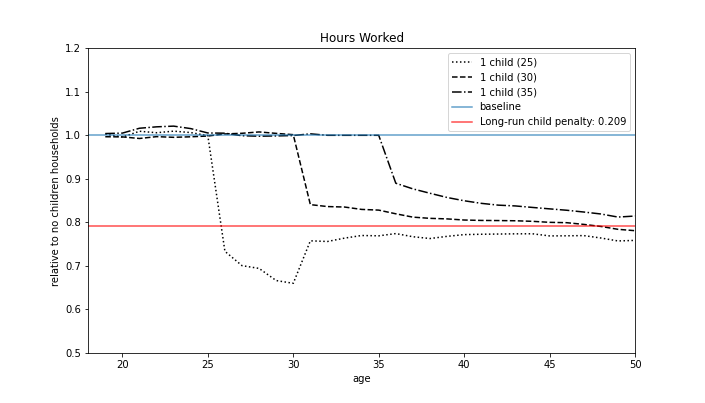
\includegraphics[width=1\linewidth]{figures/extended_model_event_hours_worked.png}
  \caption{Hours Worked}
  \label{fig:ext_model_event_hours}
\end{subfigure}
    \caption{Impact of Children (Earnings and Worked Hours)}
    \label{fig:ext_model_impact_earnings_hours}
\end{figure}

\begin{figure}[ht]
\begin{subfigure}{.5\textwidth}
  \centering
  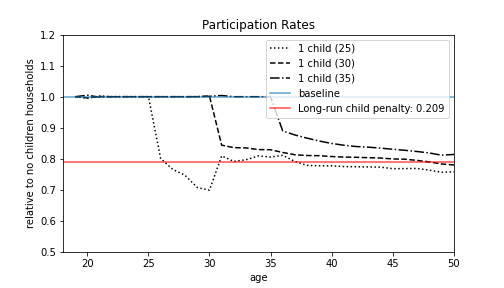
\includegraphics[width=1\linewidth]{figures/extended_model_event_participation_rates.png}
  \caption{Participation Rates}
  \label{fig:ext_model_event_partipation}
\end{subfigure}%
\begin{subfigure}{.5\textwidth}
  \centering
  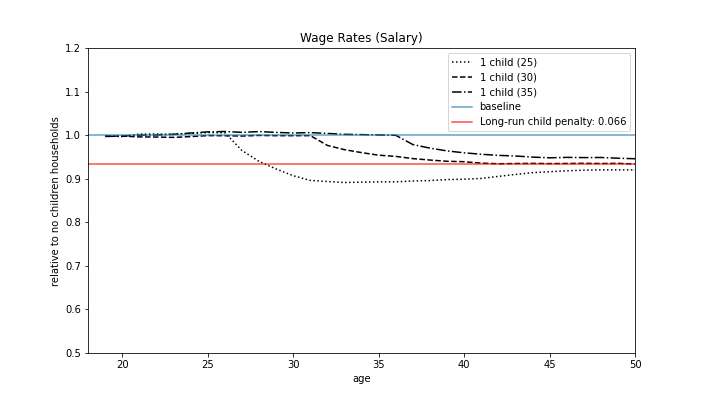
\includegraphics[width=1\linewidth]{figures/extended_model_event_wage_rates.png}
  \caption{Wage Rates}
  \label{fig:ext_model_event_wage_rates}
\end{subfigure}
    \caption{Impact of Children (Participation Rates and Wage Rates)}
    \label{fig:ext_model_impact_participation_wage}
\end{figure}


\textcite{kleven_children_2019} writes, that the event graphs they present of wage rates and hours worked is conditional on labour market participation. Figure \ref{fig:ext_model_impact_alt} shows comparable event graphs of the simulations. Here I find the reverse picture, that on average the wage rates and hours worked increase when a child is born. This effect is a consequence of selection effects. In other words, this model primarily finds effects, by letting women select out of the labour market, if they are not on high income trajectories. This clashes with the results found by \textcite{kleven_children_2019}. The RHS column of table \ref{tab:extended_results} shows the long run penalties, conditioning on labour market participation.


\begin{figure}[ht]
\begin{subfigure}{.5\textwidth}
  \centering
  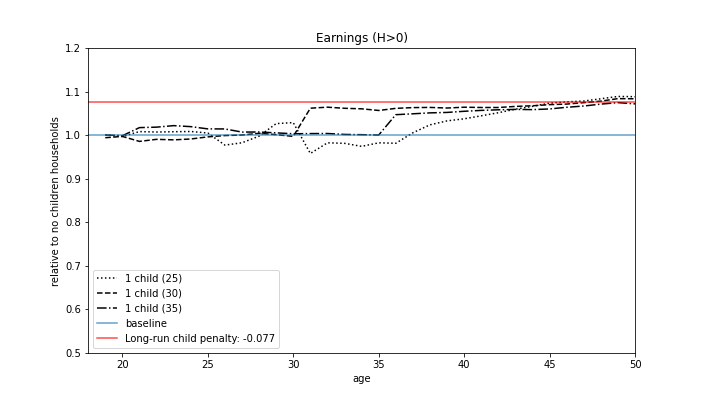
\includegraphics[width=1\linewidth]{figures/extended_model_event_earnings_H>0.png}
  \caption{Earnings Conditional on $H > 0$}
  \label{fig:ext_model_event_earnings_alt}
\end{subfigure}%
\begin{subfigure}{.5\textwidth}
  \centering
  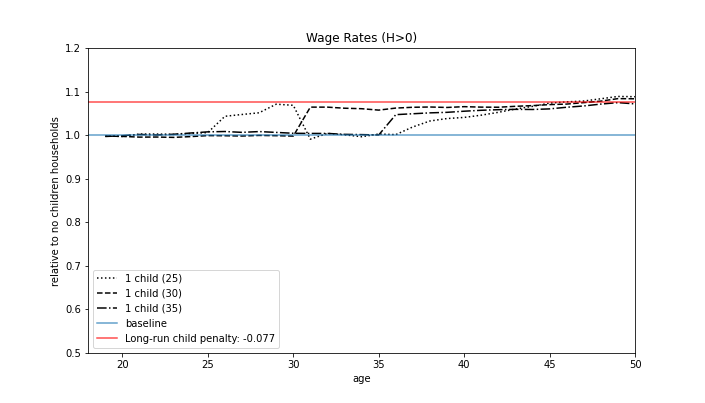
\includegraphics[width=1\linewidth]{figures/extended_model_event_wage_rates_H>0.png}
  \caption{Wage Rates Conditional on $H>0$}
  \label{fig:ext_model_event_wage_rates_alt}
\end{subfigure}
    \caption{Impact of Children Conditional on $H>0$}
    \label{fig:ext_model_impact_alt}
\end{figure}

Multiple issues can be attributed to cause these discrepancies between the model presented in this paper and the results found by \textcite{kleven_children_2019}. First, it cannot be rejected that in real Danish registry data, labour market participation is defined in a less naive way, than in this paper. This paper simply assumes, that if a woman supplies zero hours of work $(H=0)$, then said woman is unemployed. Danish registry data have a more intricate way to ascribe unemployment status to individuals, than just looking at the number of hours worked by an individual, implying that some individuals of the sample in \textcite{kleven_children_2019} could be working 0 hours. Secondly this model naively assumes an idiosyncratic wage path following a random walk. This might also contribute to the issues. In general, I believe, that to more accurately find comparable results to \textcite{kleven_children_2019} then the model, should contain more intricate family characteristics, endogenous male labour supply, a more elaborate labour market with multiple sectors and include education in the income process. This would compound to a very complex model, however as shown in this paper, using deep reinforcement learning for solving dynamic models, could make it feasible.

\begin{table}[ht]
    \centering
    \begin{tabular}{lrrr}
\toprule
                     &  Kleven et al. &  result &  result (H > 0) \\
\midrule
            Earnings &          0.194 &   0.149 &          -0.077 \\
        Hours worked &          0.097 &   0.209 &           0.000 \\
 Participation rates &          0.130 &   0.209 &             NaN \\
          Wage rates &          0.194 &   0.066 &          -0.077 \\
\bottomrule
\end{tabular}

    \caption{Long Run Penalties Comparison}
    \label{tab:extended_results}
\end{table}






\section{Conclusion}

This paper has tried to establish how reinforcement learning can be used to solve dynamic models. I show that using these solution methods allow for solving models otherwise computationally infeasible. I argue that when using such methods, there is no guarantee of finding the optimal policy, and there exists a real risk of ending up in local maxima. Furthermore have I presented an economic model of exogenous fertility and endogenous female labour supply, that can give a surprisingly good fit to data, and show comparable long term penalties for female participation rates, earnings, wage rates and hours worked to contemporary findings by \textcite{kleven_children_2019}, when a household gets a child. 

The first part of the paper, I draw on the literature of female labour supply and fertility to formulate a simple dynamic model of female labour supply and fertility, tracking households over the life cycle, where women can supply a discreet number of hours to the labour force. I use aggregate data for Statistics Denmark to calibrate the parameters of the income process. For this task I assume that the households follows a deterministic strategy with regards to labour supply. I find, the model seem to approximate the income paths of both men and women very well. Next, I present the reader for reinforcement learning and deep learning allowing the reader to have an understanding of the algorithms used for solving the models presented in this paper.  I go on to present three different solution methods: Value function Iteration using deep neural networks for value function approximation, Deep Q-learning and Double Deep Q-Learning. I find that these three solution methods have comparable performance, but the model does not seem to fit the data well! Next i formulate an extension of the inadequate model, and use Double Deep Q-learning as solution method. I estimate the extra parameters using method of simulated moments. Simulating from the model using the estimated parameters, I find that both the participation rate and the average number of supplied hours to the labour force is comparable to what is found in data. Next i compare event graphs to those found by \textcite{kleven_children_2019} and find striking similarities, finding that women do experience a real penalty when getting a child.

\clearpage

\printbibliography[heading=bibintoc]

\clearpage

\section*{Appendix}

\listoffigures
\listoftables

\begin{figure}
    \centering
    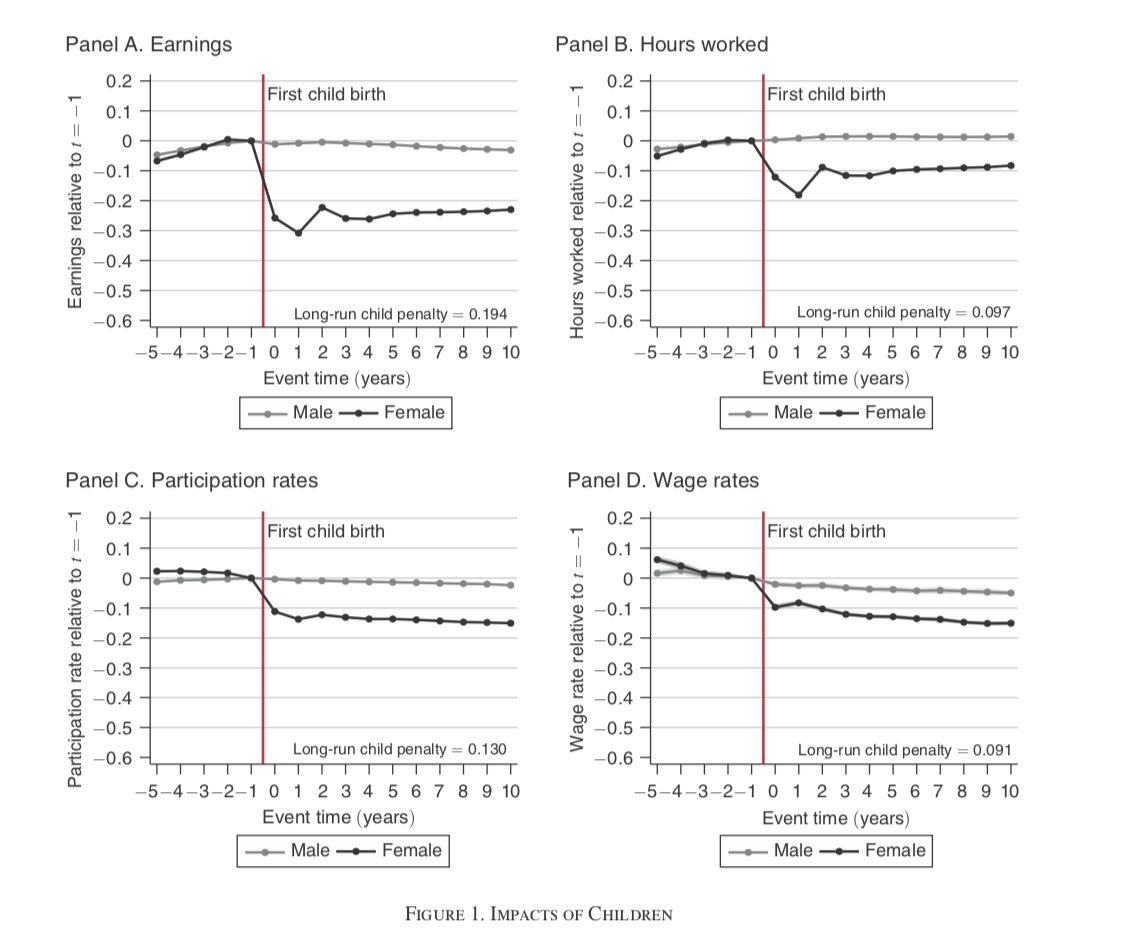
\includegraphics[scale=0.3]{figures/kleven_10_years_impact.png}
    \caption{Event Graphs of \textcite{kleven_children_2019}}
    \label{fig:my_label}
\end{figure}

\end{document}
